\documentclass[a4paper,12pt,twoside]{book} % nie: report!


% pakiety
\usepackage{polski} % lepiej to zamiast babel!
\usepackage[utf8]{inputenc} % w razie kłopotów spróbować: \usepackage[utf8x]{inputenc}
\usepackage{fancyhdr} % nagłówki i stopki
\usepackage{indentfirst} % WAŻNE, MA BYĆ!
\usepackage[pdftex]{graphicx} % to do wstawiania rysunków
\usepackage{amsmath} % to do dodatkowych symboli, przydatne
\usepackage[inner=3.5cm,outer=2cm, top=2.5cm, bottom=2.5cm]{geometry}
\usepackage{float}
\usepackage{xcolor}
% \usepackage[pdftex,
%             left=1in,right=1in,
%             top=1in,bottom=1in]{geometry} % marginsy
\usepackage{amssymb} % to też do dodatkowych symboli, też przydatne
\usepackage{pdfpages}
\usepackage{lipsum}
\usepackage{multirow}
\usepackage{listings}
\usepackage{caption}
\usepackage{booktabs}
\usepackage{subcaption}
\usepackage{xcolor}
\usepackage{url}
\usepackage{tikz} 
\usepackage{svg}
\usepackage{lipsum}  
% \usepackage{ tabularray}
\usepackage{vcell}

\graphicspath{ {./grafika/} }
\DeclareCaptionType{code}[Listing][Spis listingów] 

\definecolor{codegreen}{rgb}{0,0.6,0}
\definecolor{codegray}{rgb}{0.5,0.5,0.5}
\definecolor{codepurple}{rgb}{0.58,0,0.82}
\definecolor{backcolour}{rgb}{0.95,0.95,0.92}

\def\crnrs#1{$^\ulcorner#1_\lrcorner$}
\lstset{
	backgroundcolor=\color{backcolour},   
	commentstyle=\color{codegreen},
	keywordstyle=\color{magenta},
	numberstyle=\tiny\color{codegray},
	stringstyle=\color{codepurple},
	basicstyle=\ttfamily\footnotesize,
	breakatwhitespace=false,         
	breaklines=true,                 
	captionpos=b,                    
	keepspaces=true,                 
	numbers=left,                    
	numbersep=5pt,                  
	showspaces=false,                
	showstringspaces=false,
	showtabs=false,                  
	tabsize=2,
	float=h
}

% definicje nagłówków i stopek
\pagestyle{fancy}
% \renewcommand{\chaptermark}[1]{\markboth{#1}{}}
% \renewcommand{\sectionmark}[1]{\markright{\thesection\ #1}}
\fancyhf{}
% \fancyhead[LE,RO]{\footnotesize\bfseries\thepage}
% \fancyhead[LO]{\footnotesize\rightmark}
% \fancyhead[RE]{\footnotesize\leftmark}
% \renewcommand{\headrulewidth}{0.5pt}
% \renewcommand{\footrulewidth}{0pt}
% \addtolength{\headheight}{1.5pt}
% \fancypagestyle{plain}{\fancyhead{}\cfoot{\footnotesize\bfseries\thepage}\renewcommand{\headrulewidth}{0pt}}

\fancyhead{}
\fancyhead{}
% Set the right side of the footer to be the page number
\fancyfoot[R]{\thepage\ifodd\value{page}\else\hfill\fi}
% \fancyfoot[C]{}
% \renewcommand{\headrulewidth}{0pt}


% interlinia
\linespread{1.5}


% treść
\begin{document}
\sloppy
\thispagestyle{empty}
\includepdf{stronatytulowa}
\newpage{}

\thispagestyle{empty}
\newpage{}

\tableofcontents{}

\chapter*{Wstęp} 

Rośliny to rozległa grupa organizmów żywych, występujących na większości 
lądów na Ziemi, a także w środowisku wodnym. 
Należą do nich trawy, drzewa, kwiaty, krzewy, paprocie, mchy i wiele innych.
Istnieje około 391.000 gatunków roślin, z których zdecydowana większość,
około 369.000 (94\%), wytwarza nasiona \cite{howmanyplants}. Rośliny można znaleźć na 
całym świecie, na wszystkich kontynentach. Rośliny dostarczają znaczną część 
tlenu na świecie i stanowią podstawę
większości ekosystemów na Ziemi. Tak ważna część świata rzeczywistego
doczekała się opisanego matematycznie modelu i dalszego zastosowania w różnych rodzajach nauki, w
szczególności w informatyce. Modelowanie roślin w informatyce
jest szeroko stosowane w wielu dziedzinach, takich jak gry, przemysł filmowy, 
agrokultura i architektura. Rośliny charakteryzują się złożoną,
zwykle fraktalną strukturą, która jest trudna do modelowania.
Z tego powodu opracowano różne systemy opisywania modeli roślin,
aby uporządkować i uprościć pracę z modelowaniem drzew. Jednym z
takich systemów jest system Lindenmayera, który umożliwia opis struktur 
fraktalnych, w szczególności roślin na poziomie gramatyki formalnej.

\addcontentsline{toc}{chapter}{Wstęp}


% \chapter*{Cel pracy} 

Celem pracy jest zastosowanie i ewaluacja systemu Lindenmayera do generowania 
roślin w aplikacji do planowania przestrzeni zielonych. Specyfikacja programu 
została przygotowana we współpracy z pracownikami Instytutu Nauk Biologicznych 
Uniwersytetu Marii Curie Skłodowskiej w~Lublinie. Oprogramowanie powinno posiadać 
następujące funkcje:

\begin{itemize}
\setlength\itemsep{-0.4em}
\item[-] możliwość wyświetlania drzew w przestrzeni trójwymiarowej,
\item[-] możliwość modyfikowania drzew przy użyciu różnych parametrów,
\item[-] możliwość wyboru tekstur dla pnia drzewa i liści,
\item[-] możliwość symulacji wzrostu drzew,
\item[-] możliwość zapisywania i wczytywania drzew o określonych parametrach.

\end{itemize}


%\addcontentsline{toc}{chapter}{Cel pracy}


\chapter{System Lindenmayera} 


\section{Informacje wstępne}

\textbf{Systemy Lindenmayera (L-Systemy)} zostały wprowadzone i rozwinięte w 1968 roku
 przez Aristida Lindenmayera \cite{modelingOfPlants},
węgierskiego biologa teoretycznego i botanika z~Uniwersytetu w Utrechcie.
Lindenmayer wykorzystał L-systemy do opisu zachowania komórek roślinnych i
modelowania procesów wzrostu w rozwoju roślin.

Reguły L-systemu reprezentują rekurencję.
Prowadzi to do samopodobieństwa, a więc formy fraktalne można łatwo opisać za pomocą L-Systemu.
Modele roślin, komórek i innych form organicznych naturalnie występujących gatunków można łatwo zdefiniować za pomocą L-systemu,
ponieważ wraz ze wzrostem poziomu rekurencji forma powoli "rośnie" i staje się coraz bardziej złożona.
Systemy Lindenmayera są również popularne w symulowaniu sztucznego życia \cite{neuralStructures}.

Na rysunku \ref{fig:lsystreeexample} jest przykład zastosowania L-systemu dla stworzenia 
fraktalnej struktury, która przypomina drzewo.


\begin{figure}[H]
	\centering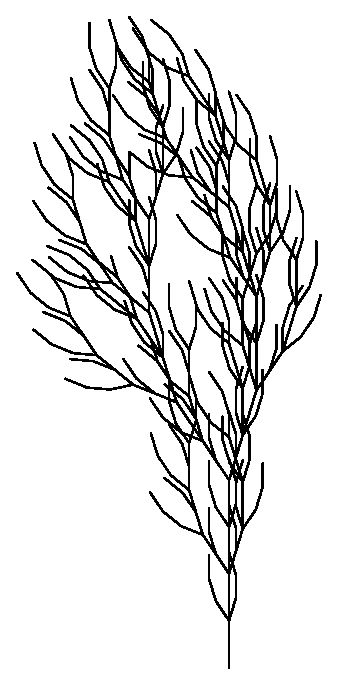
\includegraphics[height=7cm]{grafika/treefirst}
	\caption{Przykład stworzonej struktury za pomocą L-systemu}
    \label{fig:lsystreeexample}
\end{figure}

\section{Struktura L-systemu}


L-systemy są obecnie powszechnie nazywane parametrycznymi L-systemami, definiowanymi jako krotka:

\begin{gather}
	G = (V, \omega, P),
\end{gather}
gdzie

\begin{itemize}
	\item[-] V (alfabet) -- to zbiór symboli zawierający zarówno elementy, które można zastąpić (zmienne), jak i te, których nie można zastąpić ("stałe" lub "terminale"),
	\item[-] \(\omega\) (początek, aksjomat lub inicjator) -- to ciąg symboli z V, który określa stan początkowy systemu,
	\item[-] P  -- to zbiór reguł produkcji lub produktów określających sposób zastępowania zmiennych przez kombinacje stałych i innych zmiennych. Produkcja składa się z dwóch ciągów: poprzednika i następnika. Dla każdego symbolu A, który jest członkiem zbioru V i nie występuje po lewej stronie żadnego iloczynu w P, zakłada się tożsamość iloczynu A → A; symbole te nazywamy stałymi lub terminalnymi.
\end{itemize}

W standardowej wersji L-systemów reguły wnioskowania są następujące:
\begin{gather}
	v \rightarrow \omega,
\end{gather}
gdzie $v$ jest znakiem danego alfabetu $V$, $\omega \in V^* $ jest łańcuchem
znaków (ewentualnie pustym) w tym samym alfabecie.
Każdą regułę można więc interpretować jako
podział komórki $(|\omega| > 1)$, lub jej modyfikację $(|\omega| = 1)$, lub
jako jej śmierć $(|\omega| = 0)$.

Na tabeli \ref{tab:table1} przedstawiono przykład L-systemu.
\begin{table}[H]
	\caption{Przykład stworzonej struktury za pomocą L-systemu}
	\label{tab:table1}
	\begin{center}
		\begin{tabular}{|c|c|l|}
			\hline
			Alfabet & Aksjomat & Reguły \\ [0.5ex]
			\hline
			\{ \crnrs{A}, \crnrs{B}, \crnrs{F}, \crnrs{H},\crnrs{J},\crnrs{+}, \crnrs{-} \} &
			\crnrs{FB}                            &
			\crnrs{A} $\rightarrow$ \crnrs{FBFA+HFA+FB-FA} \\
			& & \crnrs{B} \(\rightarrow\) \crnrs{FB+FA-FB-JFBFA} \\
			& & \crnrs{F} \(\rightarrow\) \crnrs{} \\
			& & \crnrs{H} \(\rightarrow\) \crnrs{-} \\
			& & \crnrs{J} \(\rightarrow\) \crnrs{+}                                            \\
			\hline
		\end{tabular}
	\end{center}
\end{table}

Po zdefiniowaniu L-systemu, zaczyna ona ewoluować zgodnie ze swoimi zasadami. 
Stanem początkowym L-systemu jest jego aksjomat. 
Wraz z dalszym rozwojem ta linia opisująca stan ulegnie zmianie. 
Rozwój L-systemu odbywa się cyklicznie. W każdym cyklu rozwoju ciąg 
jest oglądany od początku do końca, symbol po symbolu. 
Dla każdego znaku wyszukiwana jest reguła, dla której ten znak 
jest poprzednikiem. Jeśli taka reguła nie zostanie znaleziona,
znak jest pozostawiony bez zmian. Innymi słowy, dla tych znaków \crnrs{X},
dla których nie istnieje reguła jawna, obowiązuje reguła domyślna: \crnrs{X} $\rightarrow$ \crnrs{X}.
Jeśli zostanie znaleziona pasująca reguła, znak poprzednika jest
zastępowany przez łańcuch następnika z tej reguły.

Dla ilustracji rozważmy następujący L-system
(nazywamy go glon (łac. \textit{algæ}), ponieważ jego rozwój
 modeluje wzrost pewnego gatunku alg) w tabeli \ref{tab:table2}:

\begin{table}[H]
	\caption{Przykład stworzonej struktury za pomocą L-systemu}
	\label{tab:table2}
	\begin{center}
		\begin{tabular}{|c|c|l|}
			\hline
			Aksjomat & Reguły \\ [0.5ex]
			\hline
			\crnrs{A} & 
			\crnrs{A} $\rightarrow$ \crnrs{B} \\

			& \crnrs{B} $\rightarrow$ \crnrs{AB} \\
			\hline
		\end{tabular}
	\end{center}
\end{table}

W tabeli \ref{tab:table3} przedstawiono stany tego L-systemu
odpowiadające pierwszym dziesięciu cyklom rozwoju systemu.

\begin{table}[H]
	\caption{Wyniki L-systemu z tabeli \ref{tab:table2} od zera do ośmiu iteracji }
	\label{tab:table3}
	\begin{center}
		\begin{tabular}{|c|l|}
			\hline
			Generacja & Stan \\ [0.5ex]
			\hline
			0 & \crnrs{A} \\
			1 & \crnrs{B} \\
			2 & \crnrs{AB} \\
			3 & \crnrs{BAB} \\
			4 & \crnrs{ABBAB} \\
			5 & \crnrs{BABABBAB} \\
			6 & \crnrs{ABBABBABABBAB} \\
			7 & \crnrs{BABABBABABBABBABABBAB} \\
			8 & \crnrs{ABBABBABABBABBABABBABABBABBABABBAB} \\
			\hline
		\end{tabular}
	\end{center}
\end{table}

Można zauważyć, że długości ciągów kodujących stan takiego L-systemu tworzą ciąg liczb Fibonacciego,
czyli ciąg liczbowy, w którym każda liczba jest równa sumie dwóch
poprzednich. Ciągami Fibonacciego będą także numery znaków A i B
w tych ciągach. Bardziej zaskakujący jest fakt, że ciąg ciągów ma
taką samą prawidłowość jak ciąg liczb Fibonacciego: każdy ciąg jest sumą
(konkatenacją) dwóch poprzednich.

Aby uzyskać stan L-systemu po określonej liczbie iteracji, 
napisałem funkcję (listing \ref{lst:lsystemfunc}), do której można wstawić aksjomat, 
zbiór reguł L-systemu oraz liczbę iteracji. 
Funkcja zwraca stan łańcucha po podanej liczbie iteracji.

\begin{lstlisting}[language=Python, caption={Funkcja, która zwraca stan systemu po określonej liczbie iteracji}, label={lst:lsystemfunc}]
	def iter(axiom: str, rules: dict, iterations: int) -> str:
    if iterations == 0: return axiom
    returnString = ''
    for i in axiom:
        if i in rules:
            returnString += rules[i]
        else:
            returnString += i
    return iter(returnString, rules, iterations-1)
\end{lstlisting}


\section{Interpretacja ciągu znaków}

W celu dalszej graficznej interpretacji otrzymanych ciągów
należy wprowadzić pojęcie grafiki żółwia. Grafika żółwia
to zasada organizacji graficznej biblioteki wyjściowej oparta 
na metaforze żółwia, wyimaginowanego 
(a w niektórych eksperymentach rzeczywistego) urządzenia 
przypominającego robota, które porusza się po ekranie 
lub papierze i obraca w zadanym kierunku, 
pozostawiając za sobą (lub opcjonalnie nie pozostawiając) 
narysowaną linię o zadanym kolorze i grubości.
Nawiązanie do żółwia inspirowane jest powstałym w latach 60. 
językiem Logo, służącym do nauki programowania, 
który wykorzystywał grafikę żółwia jako dwuwymiarowy kursor.


Interpretacja znaków polega na zdefiniowaniu operacji dla symboli
(nie jest konieczne dla wszystkich) w alfabecie. Czynności, podobnie 
jak symbole, są z kolei definiowane
przez autora systemu. Rysunek \ref{fig:interpret} przedstawia przykład interpretacji
symbolu (z kątem $\alpha = 90^\circ$ ) w następujący sposób:

\begin{figure}[H]
	\begin{center}
		\begin{tikzpicture}
			\draw [ultra thick, ->] (3,0) -- (3,3);
			\draw [thick, dashed, ->] (3,0) -- (0,0);
			\draw [thick, dashed, ->] (3,0) -- (6,0);
			\draw [thick, dotted, ->] (3,1.5) to [out=180, in=90] (1.5,0);
			\draw [thick, dotted, ->] (3,1.5) to [out=0, in=90] (4.5,0);
			\draw [fill] (3,0) circle [radius=0.1];
			\node [above] at (2.5,0.5) {-$\alpha$};
			\node [above] at (3.5,0.5) {$\alpha$};
			\node [below] at (1.5, 2.5) {\textbf{\crnrs{-}}};
			\node [below] at (4.5, 2.5) {\textbf{\crnrs{+}}};
			\node [above] at (3,3) {\textbf{\crnrs{F}}};
			\node [left] at (0,0) {\textbf{\crnrs{-F}}};
			\node [right] at (6,0) {\textbf{\crnrs{+F}}};
			\node [below] at (3,-0.1) {\textbf{$O$}};
		\end{tikzpicture}
	\end{center}
	\caption{Przykładowa interpretacja symboli}
	\label{fig:interpret}
\end{figure}

\begin{itemize}
	\item[-] \crnrs{F} oznacza przejście do przodu i narysuj linię,
	\item[-] \crnrs{-} oznacza obrót w kierunku przeciwnym do ruchu wskazówek zegara na kąt o mierze $\alpha$,
	\item[-] \crnrs{+} oznacza obrót zgodnie z ruchem wskazówek zegara o $\alpha$.
\end{itemize}

Zdefiniujemy również zbiór reguł L-systemu w tabeli \ref{tab:table4}.
Łącząc wyże wymieniony zestaw reguł z interpretacją symboli z rysunku \ref{fig:interpret}, 
otrzymujemy strukturę rekurencyjną zwaną krzywą smoka (tabela \ref{tab:table5}). 

\begin{table}[H]
	\caption{Zestaw reguł L-system dla krzywej smoka (ang. \textit{dragon curve})}
	\begin{center}
		\begin{tabular}{|c|c|l|}
			\hline
			Alfabet & Aksjomat & Reguły \\ [0.5ex]
			\hline
			\{   \crnrs{F}, \crnrs{X},\crnrs{Y} \} &
			\crnrs{FB}                            &
			\crnrs{A} $\rightarrow$ \crnrs{FBFA+HFA+FB-FA} \\
			& & \crnrs{B} \(\rightarrow\) \crnrs{FB+FA-FB-JFBFA} \\
			& & \crnrs{F} \(\rightarrow\) \crnrs{} \\
			& & \crnrs{H} \(\rightarrow\) \crnrs{-} \\
			& & \crnrs{J} \(\rightarrow\) \crnrs{+}                                            \\
			\hline
		\end{tabular}
	\end{center}
	\label{tab:table4}
\end{table}

% \begin{tblr}{
% 	colspec = {X[c]X[c,h]},
% 	stretch = 1,
% 	rowsep = 5pt,
% 	hlines = {black, 1pt},
% 	vlines = {black, 1pt}
%   }
% 	\caption{krzywa smoka w iteracji 1-7}
% 	\label{tab:table5}
% 	Iteracji & Stan \\ 
% 	1 & 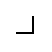
\includegraphics[scale=0.6]{grafika/example1} \\
% 	2 & 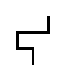
\includegraphics[scale=0.6]{grafika/example2} \\
% 	3 & 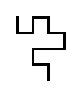
\includegraphics[scale=0.6]{grafika/example3} \\
% 	4 & 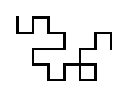
\includegraphics[scale=0.6]{grafika/example4} \\
% 	5 & 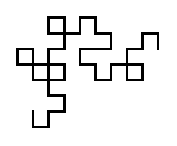
\includegraphics[scale=0.6]{grafika/example5} \\
% 	6 & 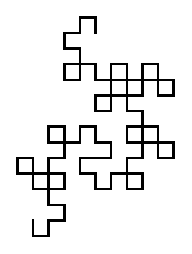
\includegraphics[scale=0.6]{grafika/example6} \\
% 	7 & 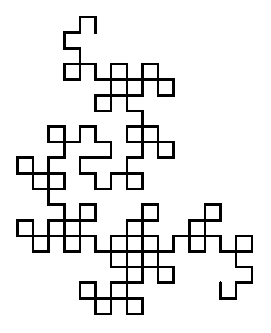
\includegraphics[scale=0.6]{grafika/example7} \\
% \end{tblr}


\begin{table}[H]
	\caption{Krzywa smoka w iteracji 1-7}
	\label{tab:table5}
		\centering
		\begin{tabular}{|c|c|}
			\hline
			Iteracji & Stan \\ [0.5ex]
			\hline
			1 &  \begin{tabular}[c]{@{}c@{}}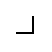
\includegraphics[scale=0.6]{grafika/example1}\\\end{tabular} \\
			\hline
			2 & \begin{tabular}[c]{@{}c@{}}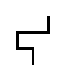
\includegraphics[scale=0.6]{grafika/example2}\\\end{tabular} \\
			\hline
			3 & \begin{tabular}[c]{@{}c@{}}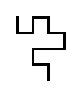
\includegraphics[scale=0.6]{grafika/example3}\\\end{tabular} \\
			\hline
			4 & \begin{tabular}[c]{@{}c@{}}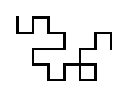
\includegraphics[scale=0.6]{grafika/example4}\\\end{tabular} \\
			\hline
			5 & \begin{tabular}[c]{@{}c@{}}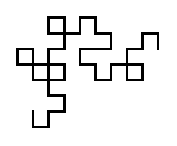
\includegraphics[scale=0.6]{grafika/example5}\\\end{tabular} \\
			\hline
			6 & \begin{tabular}[c]{@{}c@{}}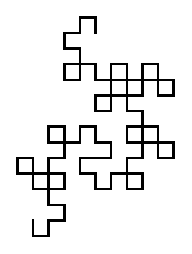
\includegraphics[scale=0.6]{grafika/example6}\\\end{tabular} \\
			\hline
			7 & \begin{tabular}[c]{@{}c@{}}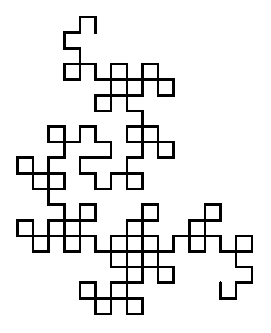
\includegraphics[scale=0.6]{grafika/example7}\\\end{tabular} \\
			\hline
		\end{tabular}
\end{table}

Widać, że po każdej iteracji struktura staje się coraz bardziej
złożona. Wynik piętnastu iteracji pokazano na rysunku \ref{fig:dragoncurve}.

\begin{figure}[H]
	\centering
	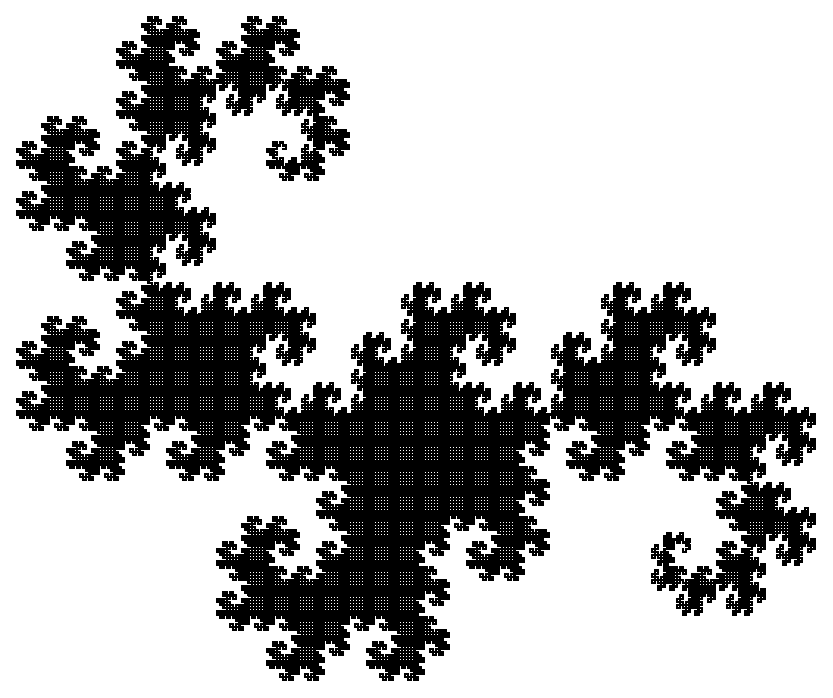
\includegraphics[scale=0.8]{grafika/example152}
	\caption{Wynik piętnastu iteracji krzywej smoka}
	\label{fig:dragoncurve}
\end{figure}

W przykładzie krzywej smoka (rysunek \ref{fig:dragoncurve}) żółw zawsze
porusza się o tę samą odległość, a jego linie mają tę samą grubość.
Jednak w świecie rzeczywistym rośliny
i drzewa mają zasadniczo strukturę rozgałęzioną. W strukturze fraktalnej
roślin każda pojedyncza gałąź może być przedstawiona jako osobna roślina,
choć w zredukowanej formie. Dlatego, aby symulować drzewa, do L-systemu 
należy dodać parametry długości i grubości linii utworzonej przez 
żółwia. 

Kolejny zestaw reguł (tabela \ref{tab:rulesTree}) demonstruje przykład tworzenia struktury 
przypominającej drzewo \cite{beautyofplants}.
W przykładzie tego L-systemu do alfabetu wprowadzane są nowe znaki. 
Ich interpretacja przez żółwia jest następująca:

\begin{itemize}
	\item[-] \crnrs{[} oznacza ``zapisać bieżący stan żółwia do stosu'',
	\item[-] \crnrs{]} oznacza ``odczytać bieżący stan żółwia do stosu'',
	\item[-] \crnrs{X} jest ignorowany przez żółwia.
\end{itemize}

W przykładzie przedstawionym w książce \cite{beautyofplants} grubość linii narysowanej
przez żółwia nie zmienia się. Rozszerzyłem przykład z podręcznika
i dodałem czynnik grubości, przez który będzie mnożona grubość 
w zależności od zagnieżdżenia gałęzi. 

W wyniku zastosowania wszystkich powyższych reguł powstaje 
struktura przypominająca drzewo (rysunek \ref{fig:treeExample})


\begin{table}[H]
	\caption{Zestaw reguł L-system dla przykładowego drzewa}
	\begin{center}
		\begin{tabular}{|c|c|l|l|}
			\hline
			Alfabet & Aksjomat & Reguły  & Konstanty \\ [0.5ex]
			\hline
			\{   \crnrs{F}, \crnrs{X}, \crnrs{[}, \crnrs{]} \} & 
			\crnrs{X}                            &
			\crnrs{X} $\rightarrow$ \crnrs{F[+X]F[-X]+X} &
			Kąt powrotu = $20^\circ$ \\
			& & \crnrs{F} $\rightarrow$ \crnrs{F} & 
			Grubość linii = 6px \\
			& & & Czynnik grubości = 0.5 \\
			\hline
		\end{tabular}
	\end{center}
	\label{tab:rulesTree}
\end{table}


\begin{figure}[H]
	\centering
	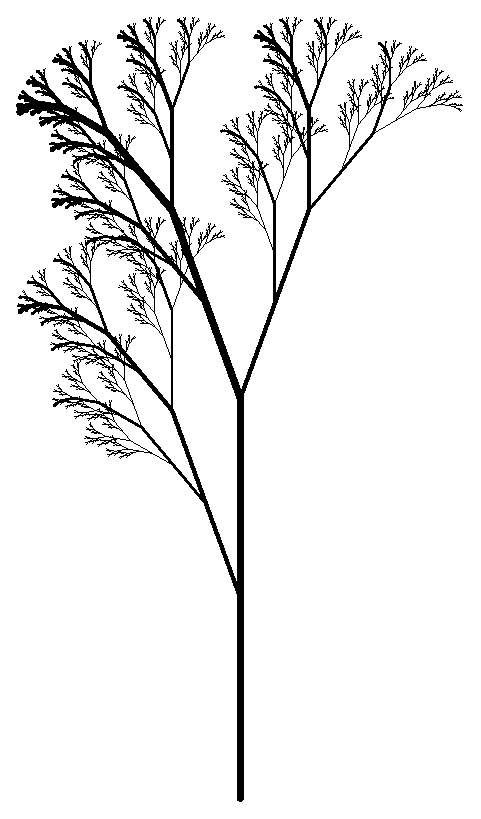
\includegraphics[scale=0.8]{grafika/treeExample}
	\caption{Utworzona struktura na podstawie reguł z tabeli \ref{tab:rulesTree}}
	\label{fig:treeExample}
\end{figure}


% Również, w przypadku zdefiniowanych reguł l-systemu w tabeli \ref{tab:table4}, 
% zastosowanie powyższych reguł daje za każdym razem taki sam wynik.
% Jednak w świecie rzeczywistym prawie niemożliwe jest napotkanie dwóch
% identycznych struktur fraktalnych. Wiele czynników świata 
% rzeczywistego ma wpływ na końcowy rezultat każdej konstrukcji. 
% Dlatego, aby symulować prawdziwe rośliny, musimy dodać do l-systemu 
% losowość.  

\subsection{Trójwymiarowe generowanie drzew}

Aby utworzyć trójwymiarowe drzewa, należy zdefiniować symbole dla żółwia, 
który będzie odpowiedzialny za obroty w przestrzeni trójwymiarowej. 
Jednym ze sposobów byłoby zdefiniowanie obrotów żółwia na każdej osi (X, Y, Z), 
a także możliwość ustawienia kąta obrotu. Dzięki temu żółw może poruszać się we 
wszystkich możliwych kierunkach. Podczas budowania drzewa, w momencie gdy gałąź 
się rozgałęzia, należy, podobnie jak w przypadku 2D, ustawić kąty dla każdej z 
nowych gałęzi. Lindenmayer sugeruje użycie trzech wektorów 
do reprezentowania kierunku żółwia (przód, lewo i góra) \cite{beautyofplants}.

W tym przypadku obroty żółwia będą reprezentowane przez 
następujące równanie:

\begin{gather}
	\left[ \; \overrightarrow{H}' \; \overrightarrow{L}' \; \overrightarrow{U}' \; \right] 
	= \left[ \; \overrightarrow{H} \; \overrightarrow{L} \;  \overrightarrow{U} \; \right] R,
\end{gather}

gdzie 
\begin{itemize}
	\item[-] H jest wektorem wskazującym górę żółwia, 
	\item[-] L jest wektorem wskazującym lewą stronę żółwia, 
	\item[-] F jest wektorem wskazującym przód żółwia,
	\item[-] R jest macierzą trójwymiarową.
\end{itemize}
 Macierz R, w zależności od osi obrotu, 
może wyglądać w następujący sposób:

\begin{gather}
	R_{H}(\alpha) =  
	\begin{bmatrix}
		1 & 0 & 0 \\
		0 & \cos{\alpha} & -\sin{\alpha}   \\
		0 & \sin{\alpha} & \cos{\alpha}  
	\end{bmatrix}
\end{gather}

\begin{gather}
	R_{L}(\alpha) =  
	\begin{bmatrix}
		\cos{\alpha} & 0 & -\sin{\alpha}   \\
		0 & 1 & 0 \\
		\sin{\alpha} & 0 &  \cos{\alpha}
	\end{bmatrix}
\end{gather}

\begin{gather}
	R_{U}(\alpha) =  
	\begin{bmatrix}
		\cos{\alpha} & \sin{\alpha} & 0   \\
		-\sin{\alpha} & \cos{\alpha} &  0 \\
		0 & 0 & 1
	\end{bmatrix}
\end{gather}



\chapter{Implementacja} 

W zakresie implementacji stworzyłem oprogramowanie, które pozwala na 
wizualizację przyległego terenu do nieruchomości w trójwymiarowej 
przestrzeni, na której można umieścić drzewa. Drzewa można 
zmieniać za pomocą różnych parametrów i symulować ich wzrost.

\section{Wykorzystane narzędzia}

\subsection{Język i zintegrowane środowisko programistyczne}

Do stworzenia programu wykorzystałem język programowania 
C++ w standardzie 17. Użyłem Qt Creator w wersji 6.0.1 jako 
zintegrowanego środowiska programistycznego.

Stworzone oprogramowanie wykorzystuje język C++ dla całej logiki aplikacji.

\subsection{Biblioteka Proctree}

Proctree.js to biblioteka dla języka programowania javascript, 
która pozwala na tworzenie drzewa jako siatki wierzchołków \cite{proctreejs}.
Biblioteka posiada dużą liczbę parametrów, które wpływają na 
ostateczny wynik drzewa. Autorem biblioteki jest brytyjski 
programista Paul Brunt. Później fiński programista Jari Komppa 
zrobił port tej biblioteki dla C++. Biblioteka w wersji C++ jest szybsza \cite{proctree}.

Biblioteka Proctree jest głównym narzędziem do tworzenia siatki wierzchołków,
normalnych i mapowania UV dla drzewa w programie.


\subsection{Biblioteka Nlohmann JSON}

Nlohmann Json to biblioteka do obsługi danych formatu json \cite{nlohmannjson}.
Biblioteka ma wiele zalet: Intuicyjna syntaktyka, Łatwa integracja,
Wydajność pamięci, Szybkość. Autorem biblioteki jest 
niemiecki programista Niels Lohmann.

Biblioteka Nlohmann Json jest używana w programie do zapisywania i 
ładowania parametrów drzewa w postaci pliku json.

\subsection{OpenGL}

OpenGL jest specyfikacją definiującą niezależny od
platformy interfejs programowania aplikacji do pisania 
aplikacji wykorzystujących grafikę komputerową 2D i 3D. 
Twórcą jest amerykańska firma Silicon Graphics. OpenGL pozwala na tworzenie 
złożonych scen 3D za pomocą prymitywów. Wykorzystuje do tego zasoby 
karty graficznej. Wykorzystywany jest do 
tworzenia gier komputerowych, wirtualnej rzeczywistości, w projektowaniu.

Powstałe oprogramowanie wykorzystuje OpenGL wersji 3.3 Core do renderowania trójwymiarowej 
przestrzeni i drzew.

\section{Funkcjonalność aplikacji}

Stworzone oprogramowanie posiada szereg funkcji, które pozwalają na 
zaprojektowanie rozmieszczenia drzew w otoczeniu przy budynku. 

Na rysunku \ref{fig:screenmainwindow} można zaobserwować główne okno programu. 
Konwencjonalnie okno główne można podzielić na dwa obszary -- 
obszar ustawień i obszar roboczy.

Część ustawień znajduje się po lewej i dolnej stronie okna. 
Obszar roboczy zajmuje większość okna i znajduje się po prawej stronie okna.

Obszar ustawień obejmuje:
\begin{enumerate}
	\item suwak do regulacji drzew,
	\item suwak do zmiany wieku drzewa,
	\item lista utworzonych drzew,
	\item przycisk symulacji wzrostu drzew,
	\item przycisk do zmiany tekstur,
	\item pasek menu.
\end{enumerate}

\begin{figure}[H]
	\centering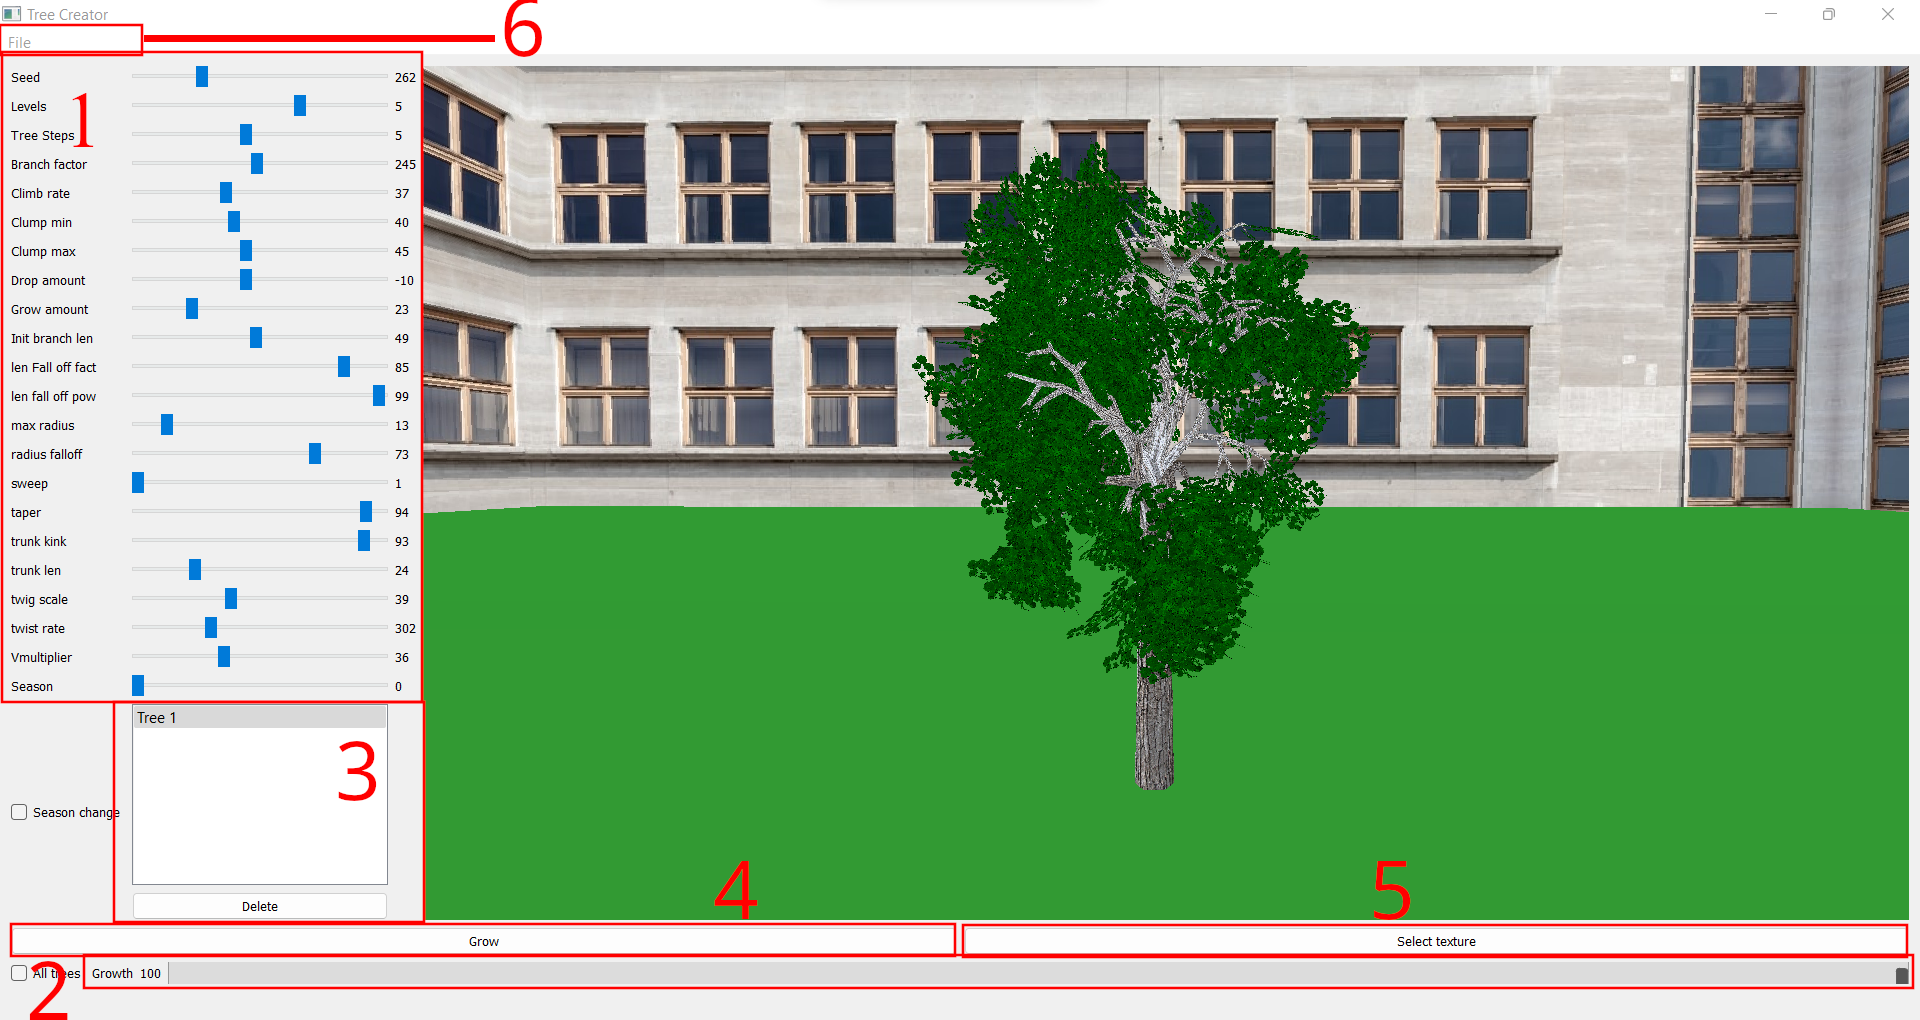
\includegraphics[width=15.5cm]{grafika/program/main2.png}
	\caption{Główne okno programu}
    \label{fig:screenmainwindow}
\end{figure}

Obszar roboczy to trójwymiarowa przestrzeń, która symuluje obszar 
wokół budynku drzewa. Kamerę można przesuwać za pomocą klawiatury. 
Klawisze W, A, S, D służą do poruszania się odpowiednio do przodu, 
w lewo, do tyłu i w prawo. Klawisz Shift służy do poruszania się wyżej. 
Aby obniżyć kamerę niżej, użyj klawisza Alt. 
Kamerę można obracać za pomocą myszy z wciśniętym lewym przyciskiem.  


\subsection{Planowanie drzew}

Aby posadzić drzewa, najpierw za pomocą myszy i klawiatury 
ustawiamy kamerę tak, aby widoczny był obszar, w którym chcemy 
posadzić drzewko (rysunek \ref{fig:placeTree}). Następnie umieszczamy kursor w miejscu, w którym 
chcemy posadzić drzewo i klikamy prawym przyciskiem myszy (rysunek \ref{fig:placeTree2}).


\begin{figure}[H]
	\centering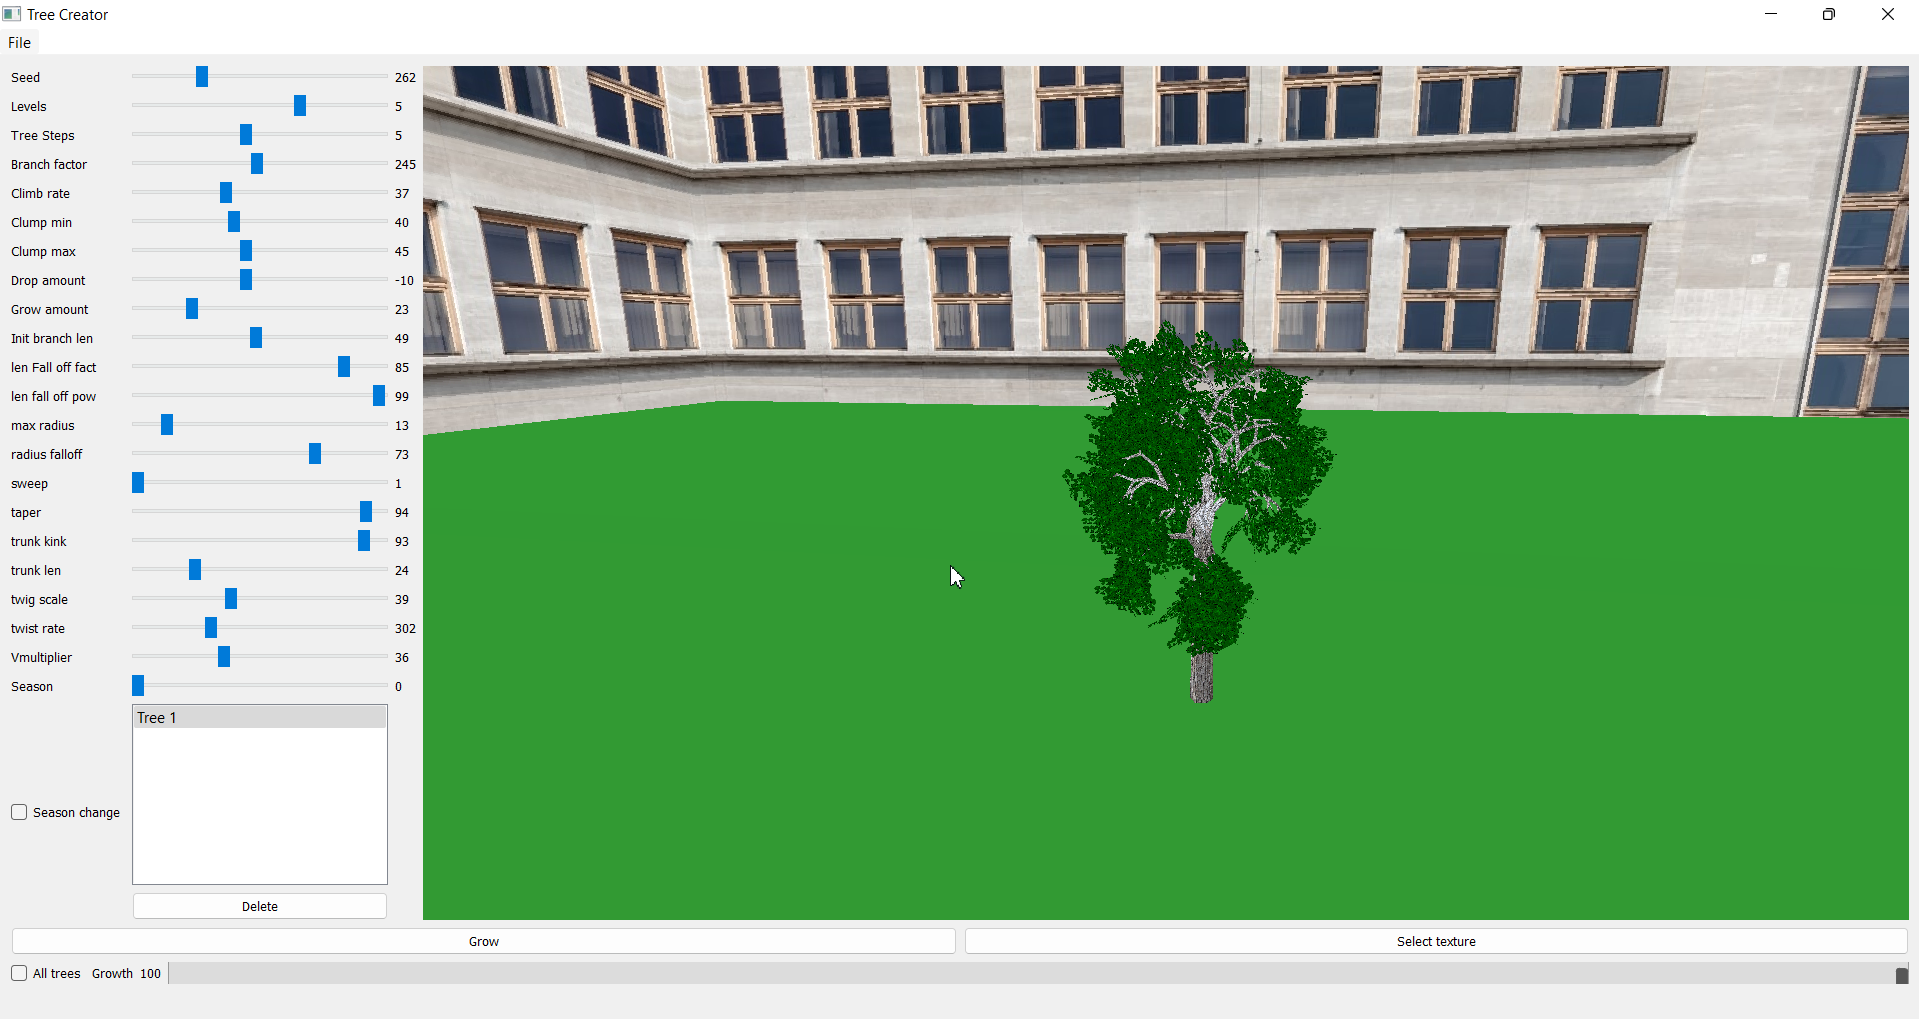
\includegraphics[width=15.5cm]{grafika/program/placeTree.png}
	\caption{Okno programu przed posadzeniem drzewa}
    \label{fig:placeTree}
\end{figure}

\begin{figure}[H]
	\centering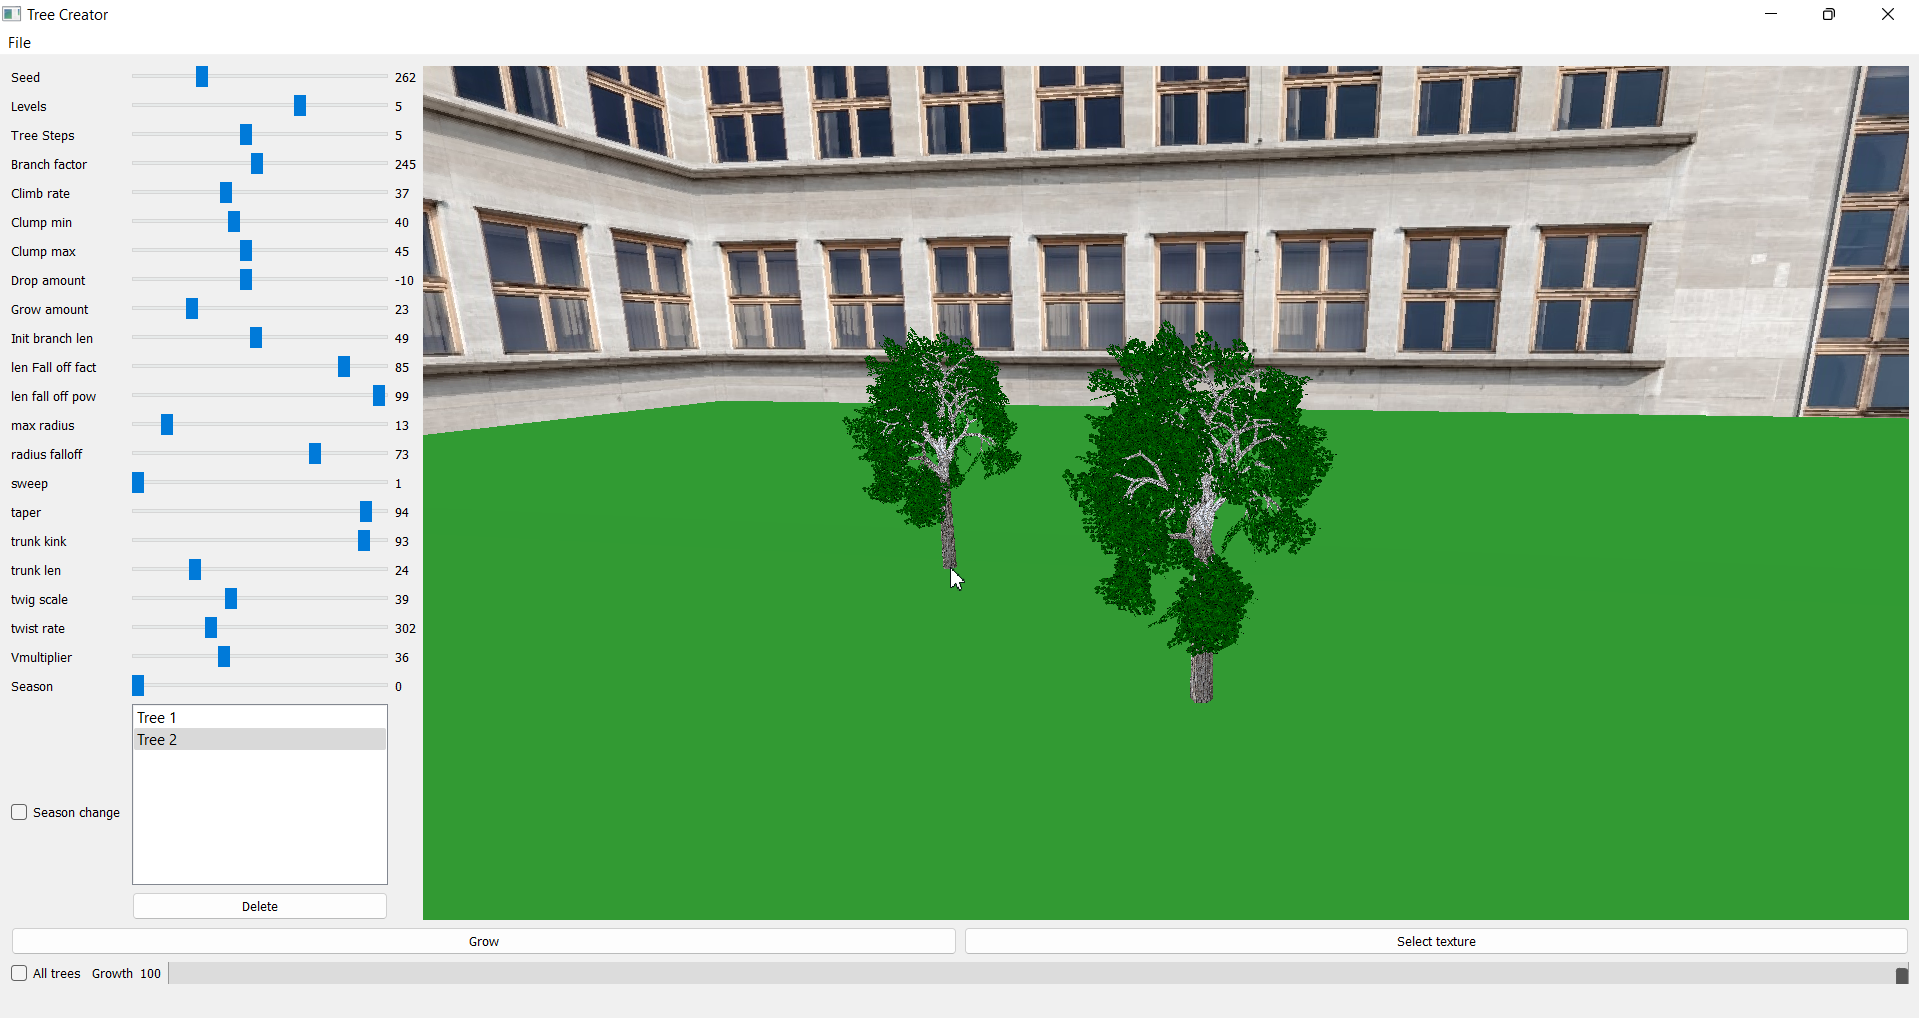
\includegraphics[width=15.5cm]{grafika/program/placeTree2.png}
	\caption{Okno programu po posadzeniu drzewa}
    \label{fig:placeTree2}
\end{figure}

Nie ma ograniczeń co do liczby drzew w programie, 
ale należy pamiętać, że duża liczba drzew może wpłynąć na wydajność, 
a w szczególności na symulację wzrostu. Rysunek \ref{fig:50trees} pokazuje 
50 posadzonych drzew.

\begin{figure}[H]
	\centering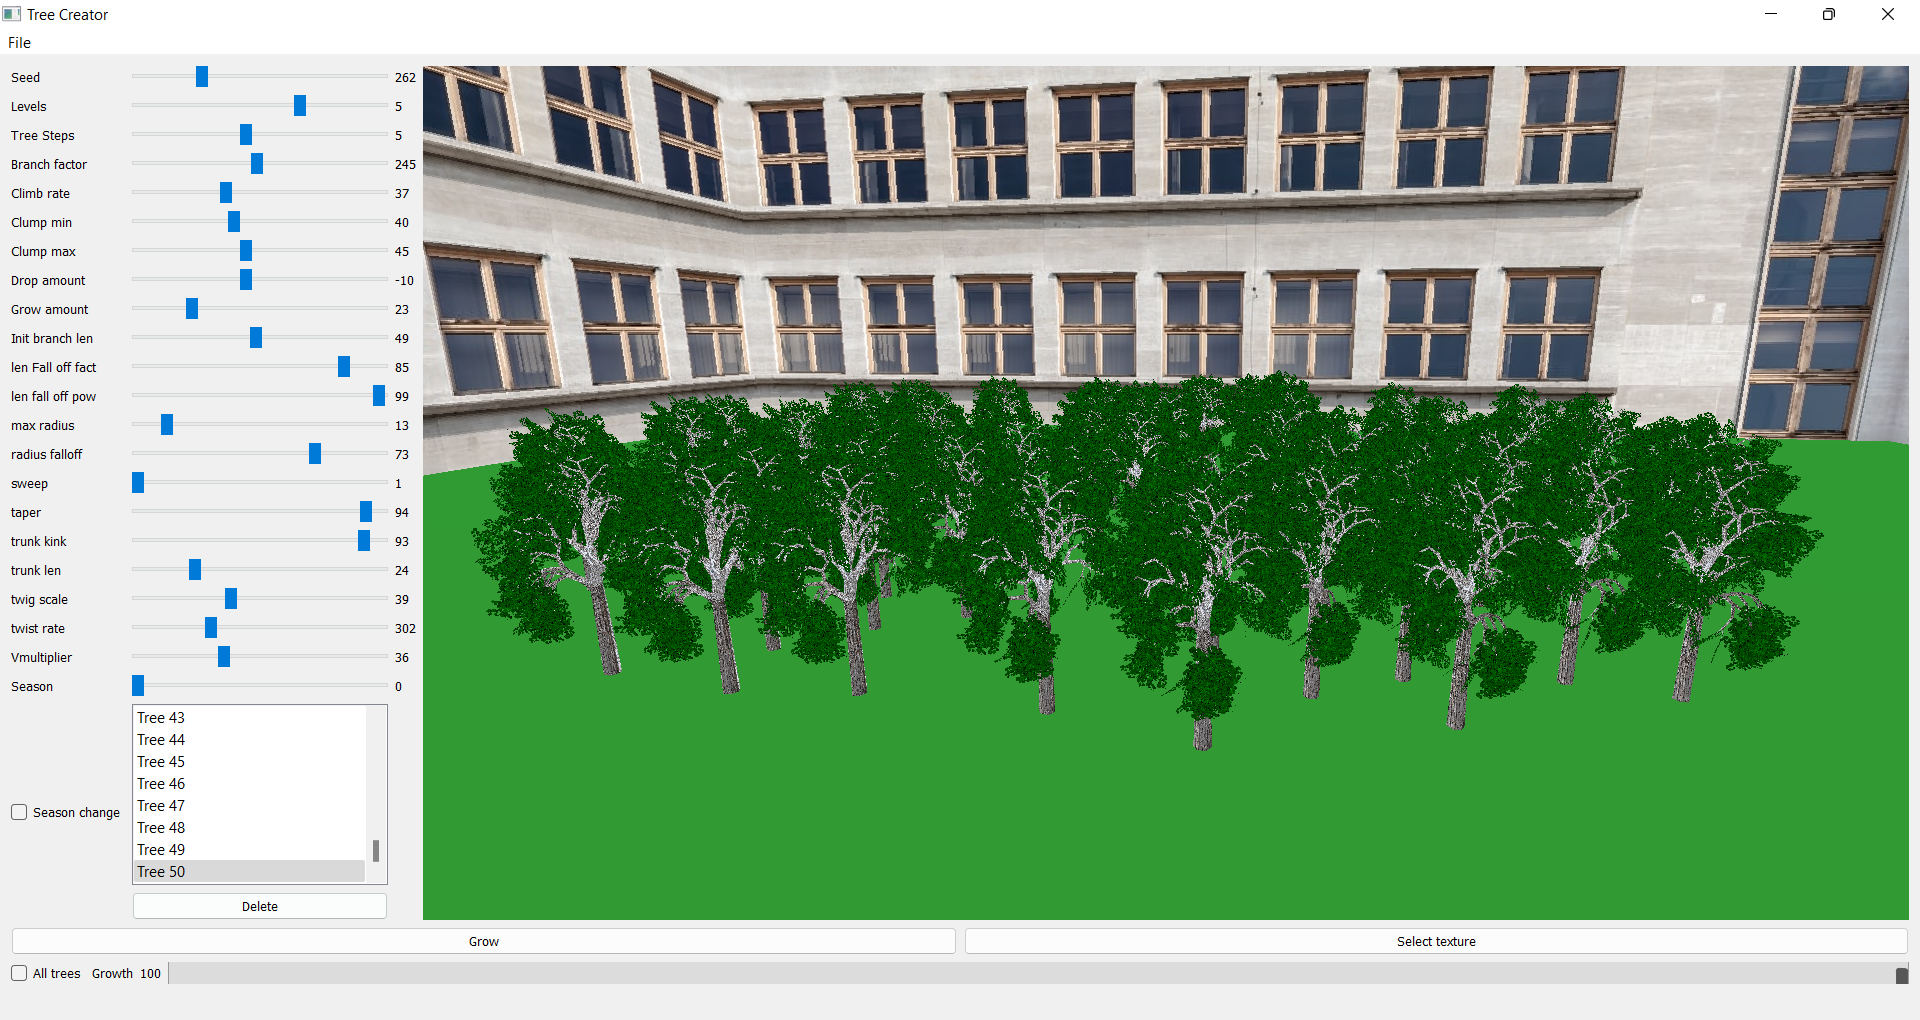
\includegraphics[width=15.5cm]{grafika/program/50trees.png}
	\caption{50 posadzonych drzew}
    \label{fig:50trees}
\end{figure}

\subsection{Symulacja wzrostu}

Na potrzeby demonstracji ustawiłem trzy drzewa i 
zmieniłem ich parametry, aby były różne (rysunek \ref{fig:beforeGrow}).

\begin{figure}[H]
	\centering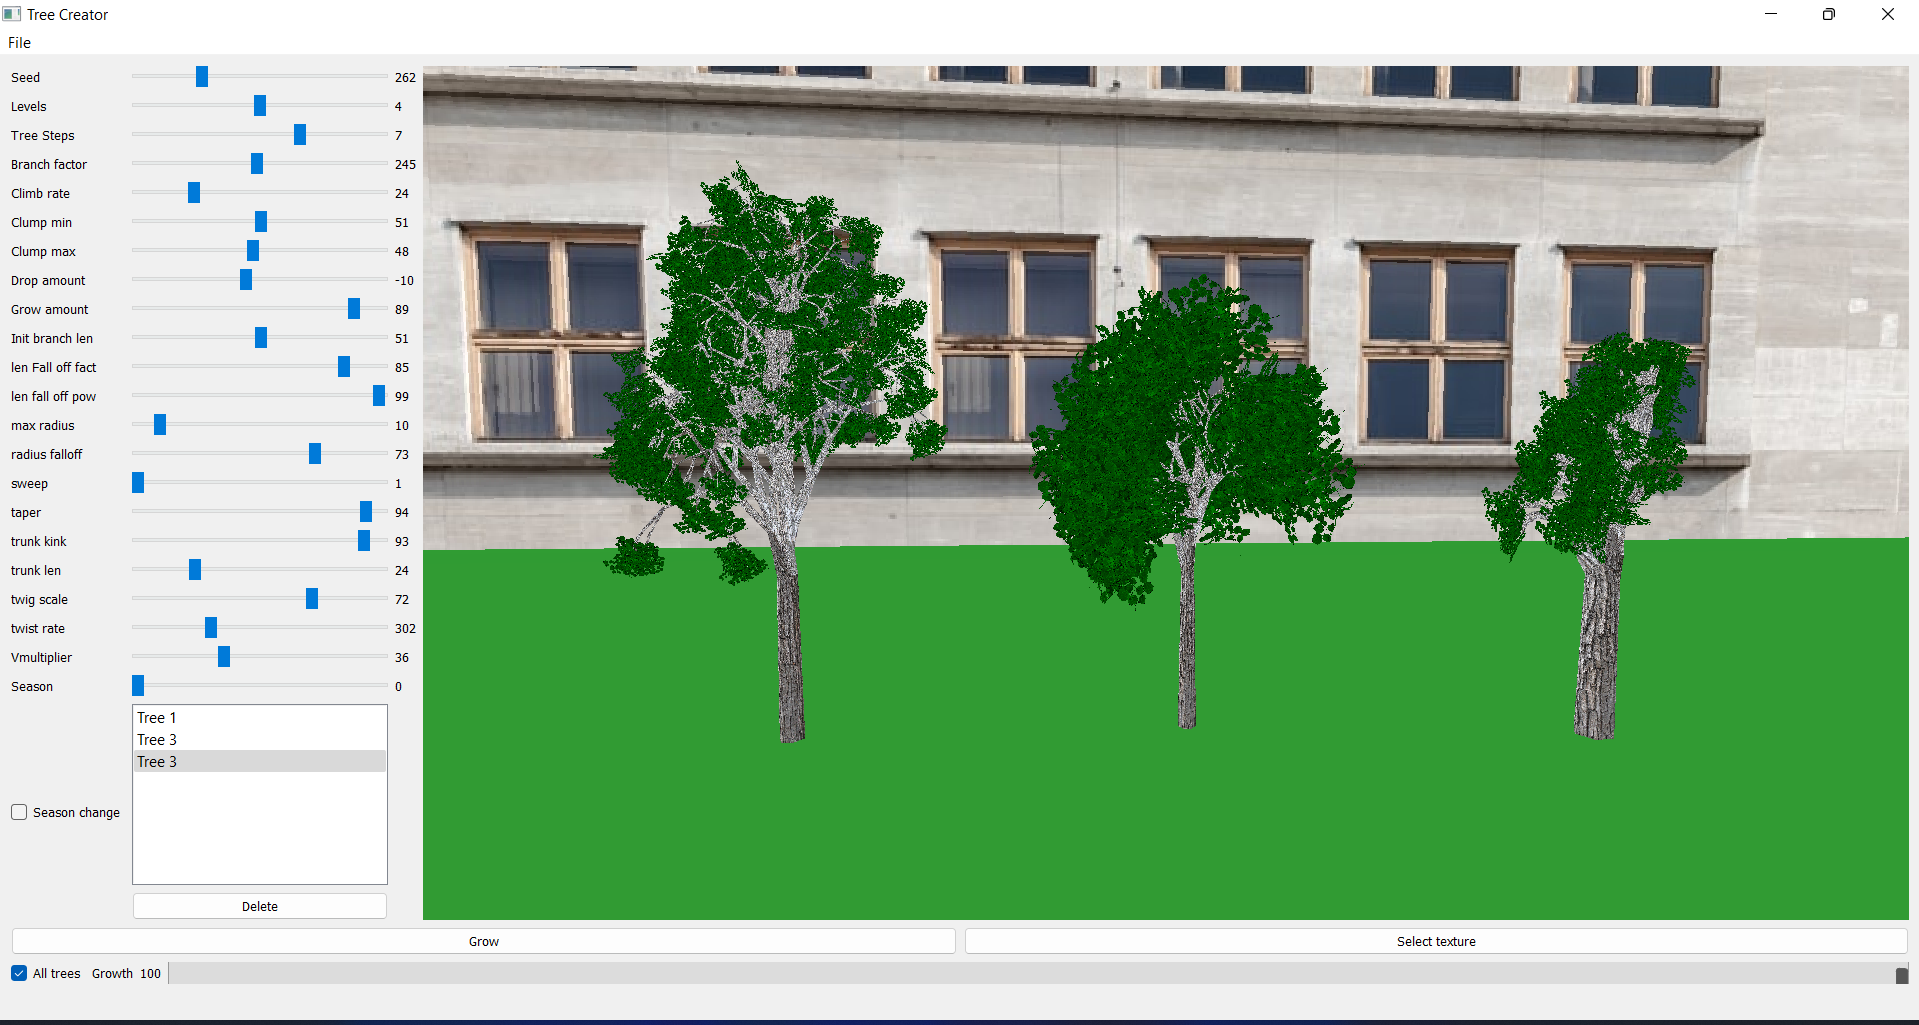
\includegraphics[width=15.5cm]{grafika/program/beforeGrow.png}
	\caption{Trzy różnych drzewa}
    \label{fig:beforeGrow}
\end{figure}

Symulacja wzrostu może odbywać się na dwa sposoby: 
ręcznie, poprzez ustawienie ``wieku'' drzewa (rysunek \ref{fig:oneTree}, \ref{fig:percentGrow}), 
oraz automatycznie, poprzez naciśnięcie przycisku ``Rosnąć'' \textit{(ang. Grow)} (rysunek \ref{fig:growAll}). 
Każda z tych metod ma dwa tryby: zmiana wzrostu pojedynczego 
wybranego drzewa (rysunek \ref{fig:oneTree}) lub zmiana wzrostu wszystkich drzew (rysunki \ref{fig:percentGrow}, \ref{fig:growAll}). 
Tryb jest przełączany za pomocą przycisku wyboru ``Wszystkie drzewa'' \textit{(ang. All trees)}. 

\begin{figure}[H]
	\centering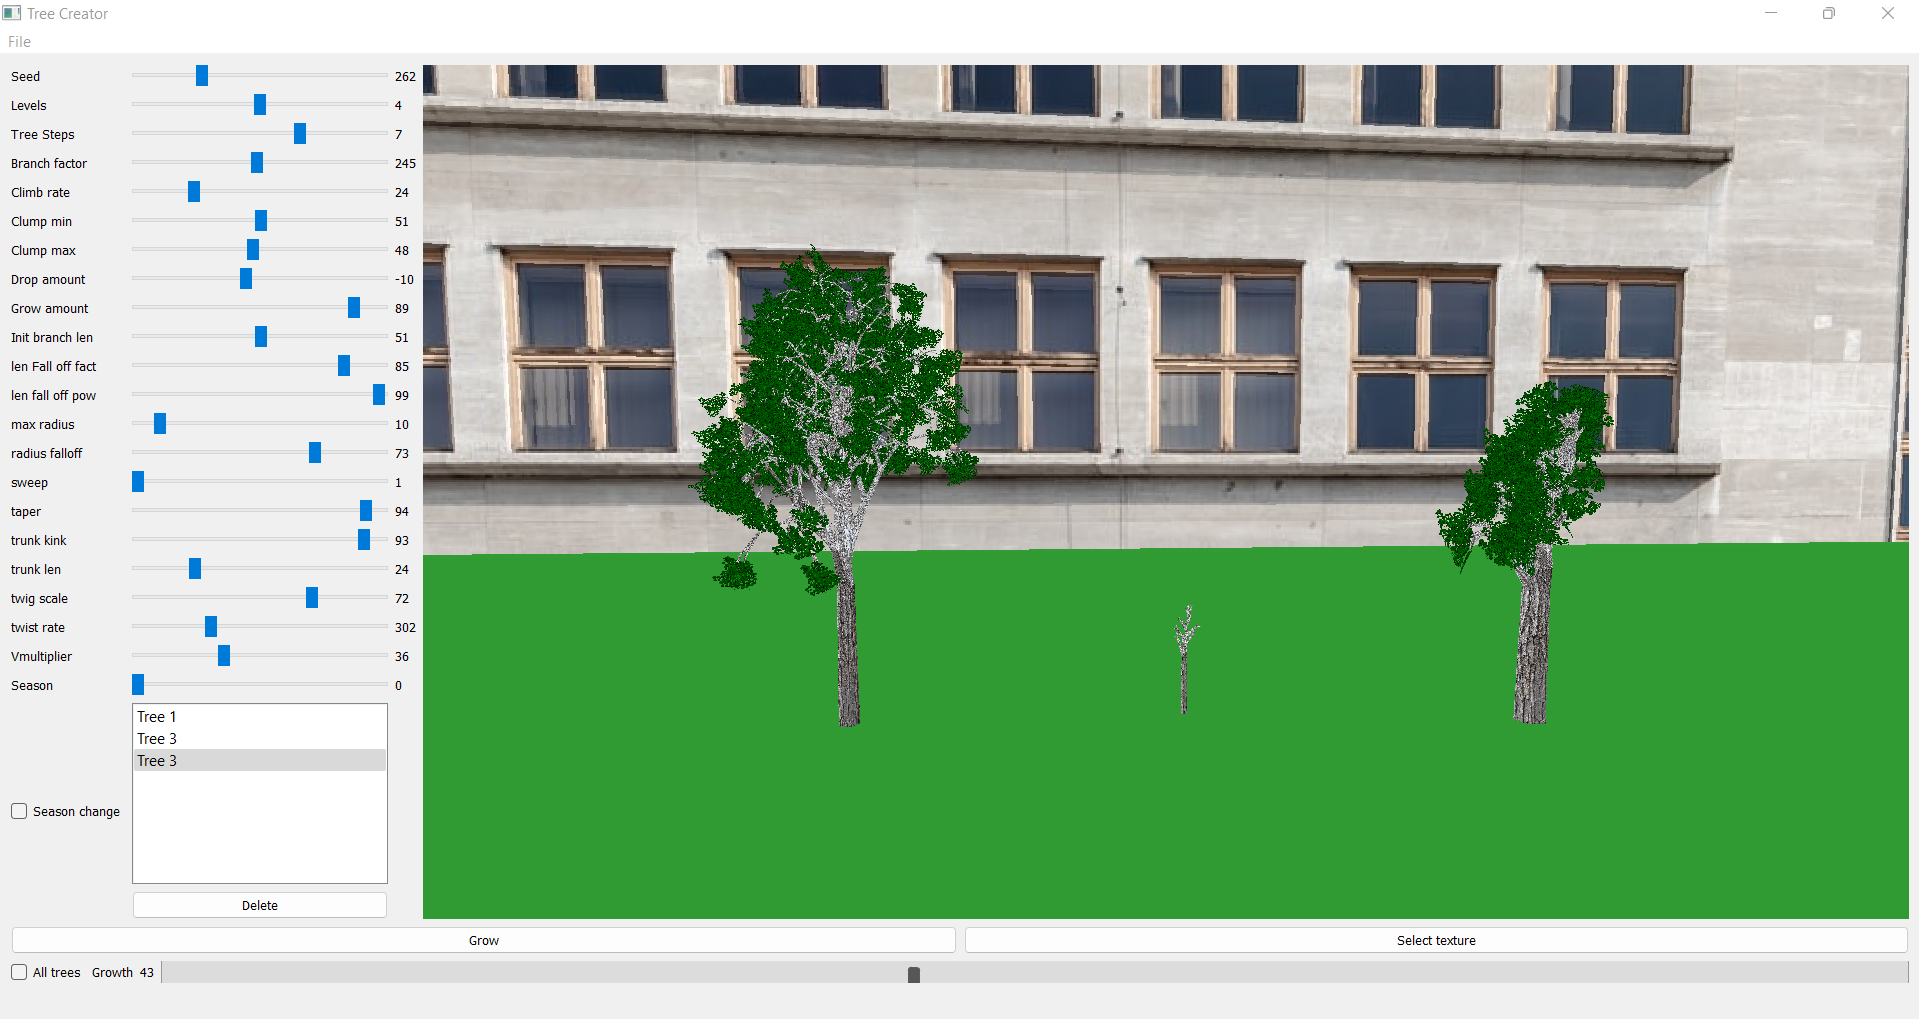
\includegraphics[width=15.5cm]{grafika/program/oneTreeGrow.png}
	\caption{Ręczna zmiana wzrostu jednego drzewa}
    \label{fig:oneTree}
\end{figure}

\begin{figure}[H]
	\centering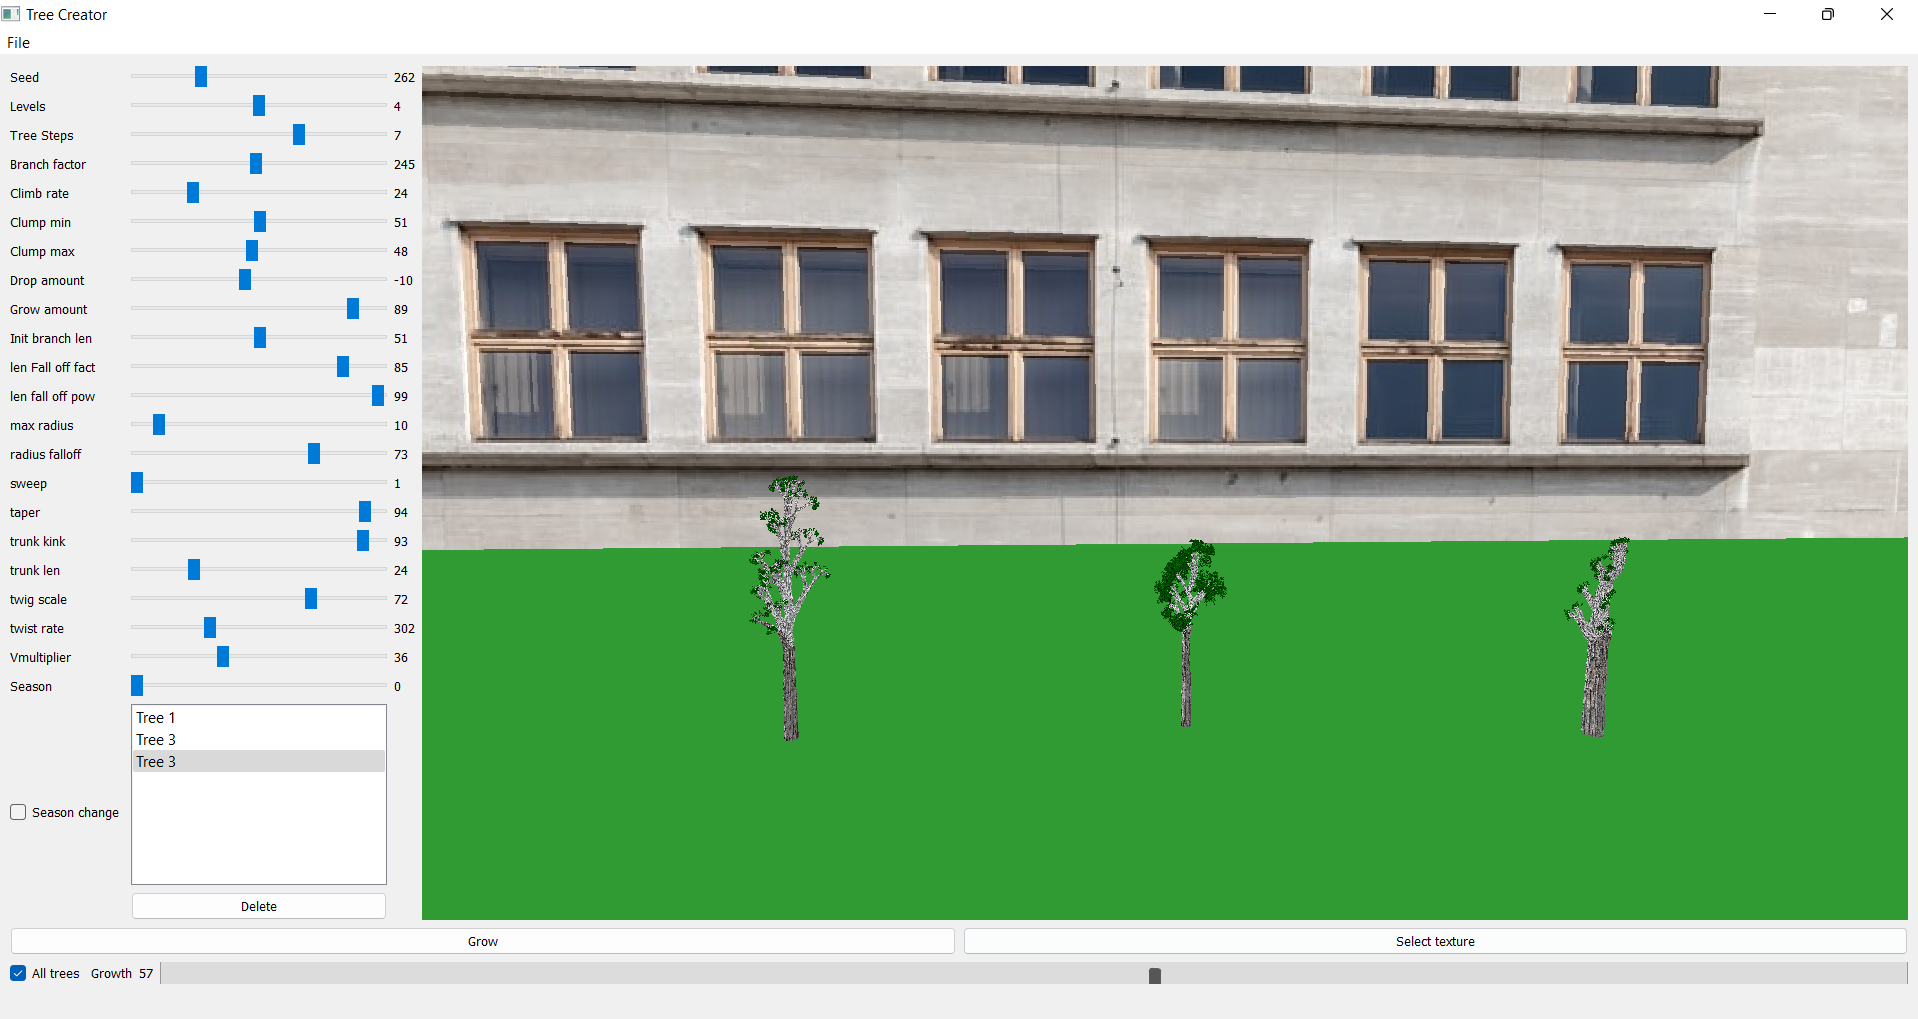
\includegraphics[width=15.5cm]{grafika/program/percentGrow.png}
	\caption{Ręczna zmiana wzrostu wszystkich drzew}
    \label{fig:percentGrow}
\end{figure}


% \begin{figure}[H]
% 	\centering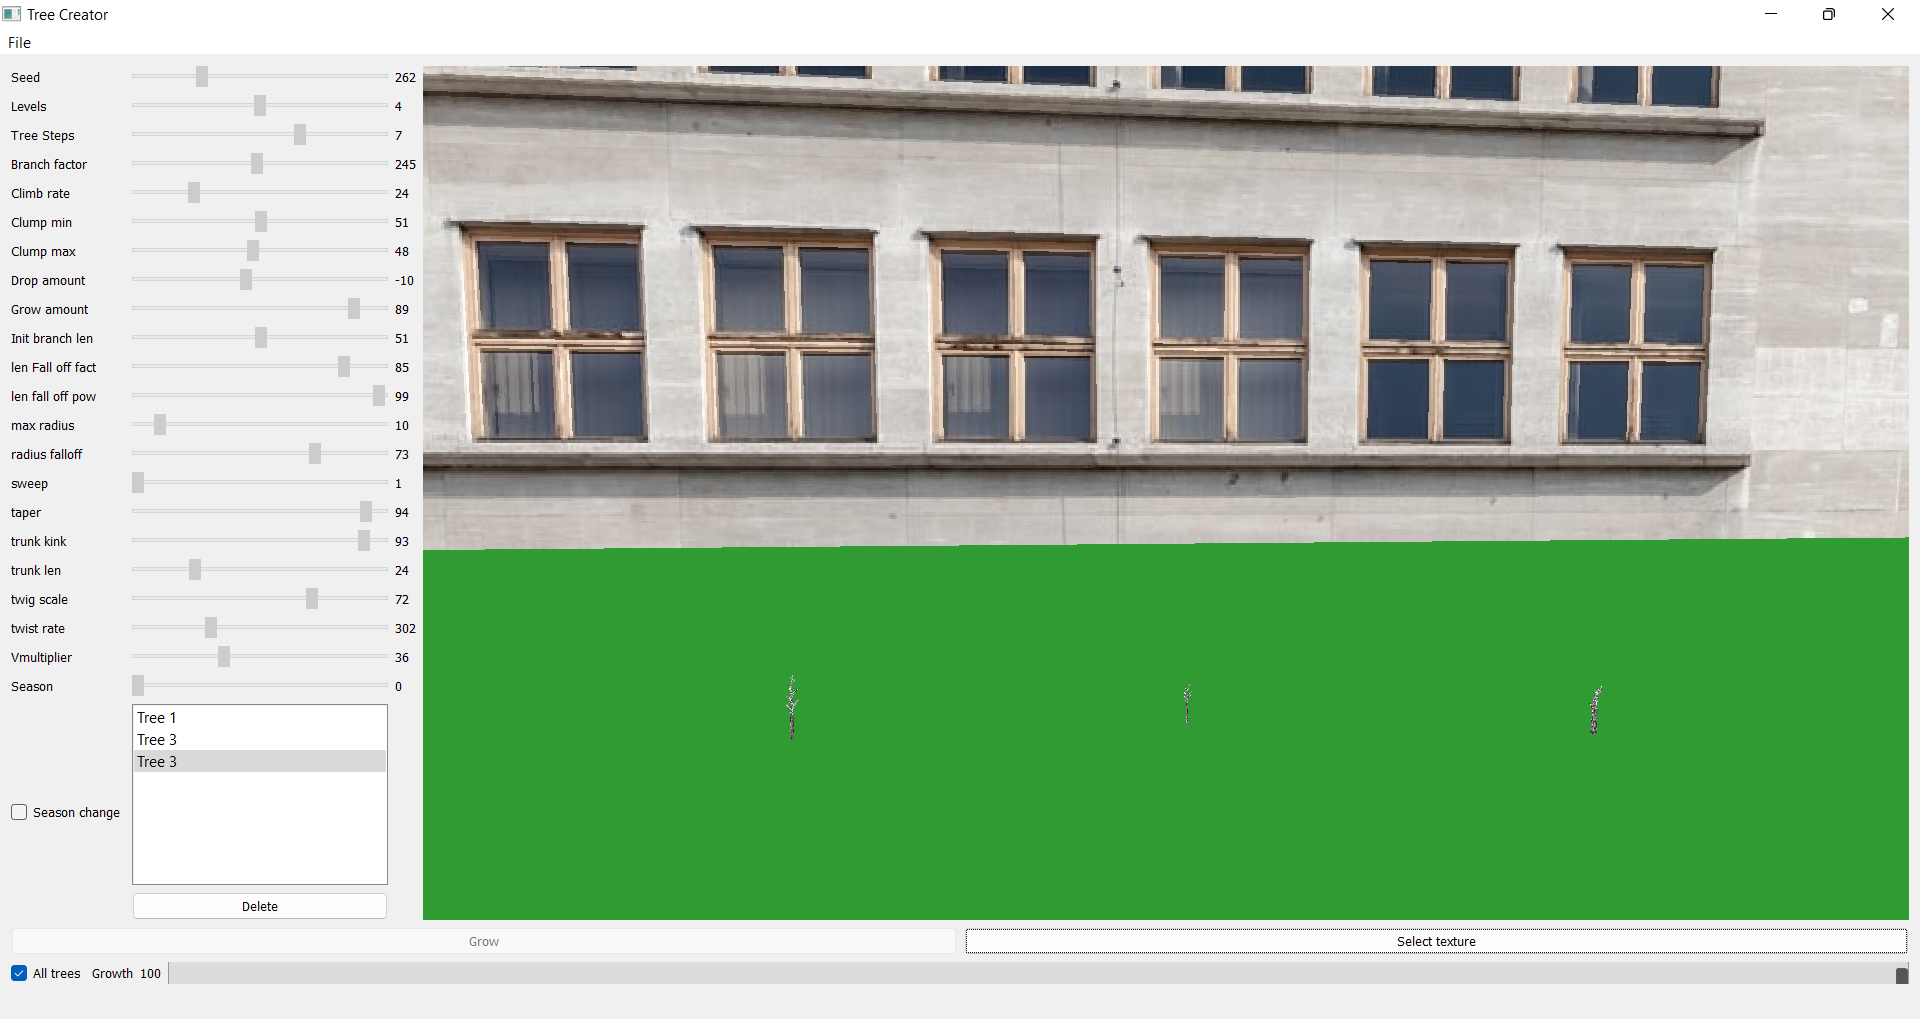
\includegraphics[width=15.5cm]{grafika/program/grow1.png}
% 	\caption{Początek automatycznego wzrostu drzew}
%     \label{fig:grow1}
% \end{figure}

% \begin{figure}[H]
% 	\centering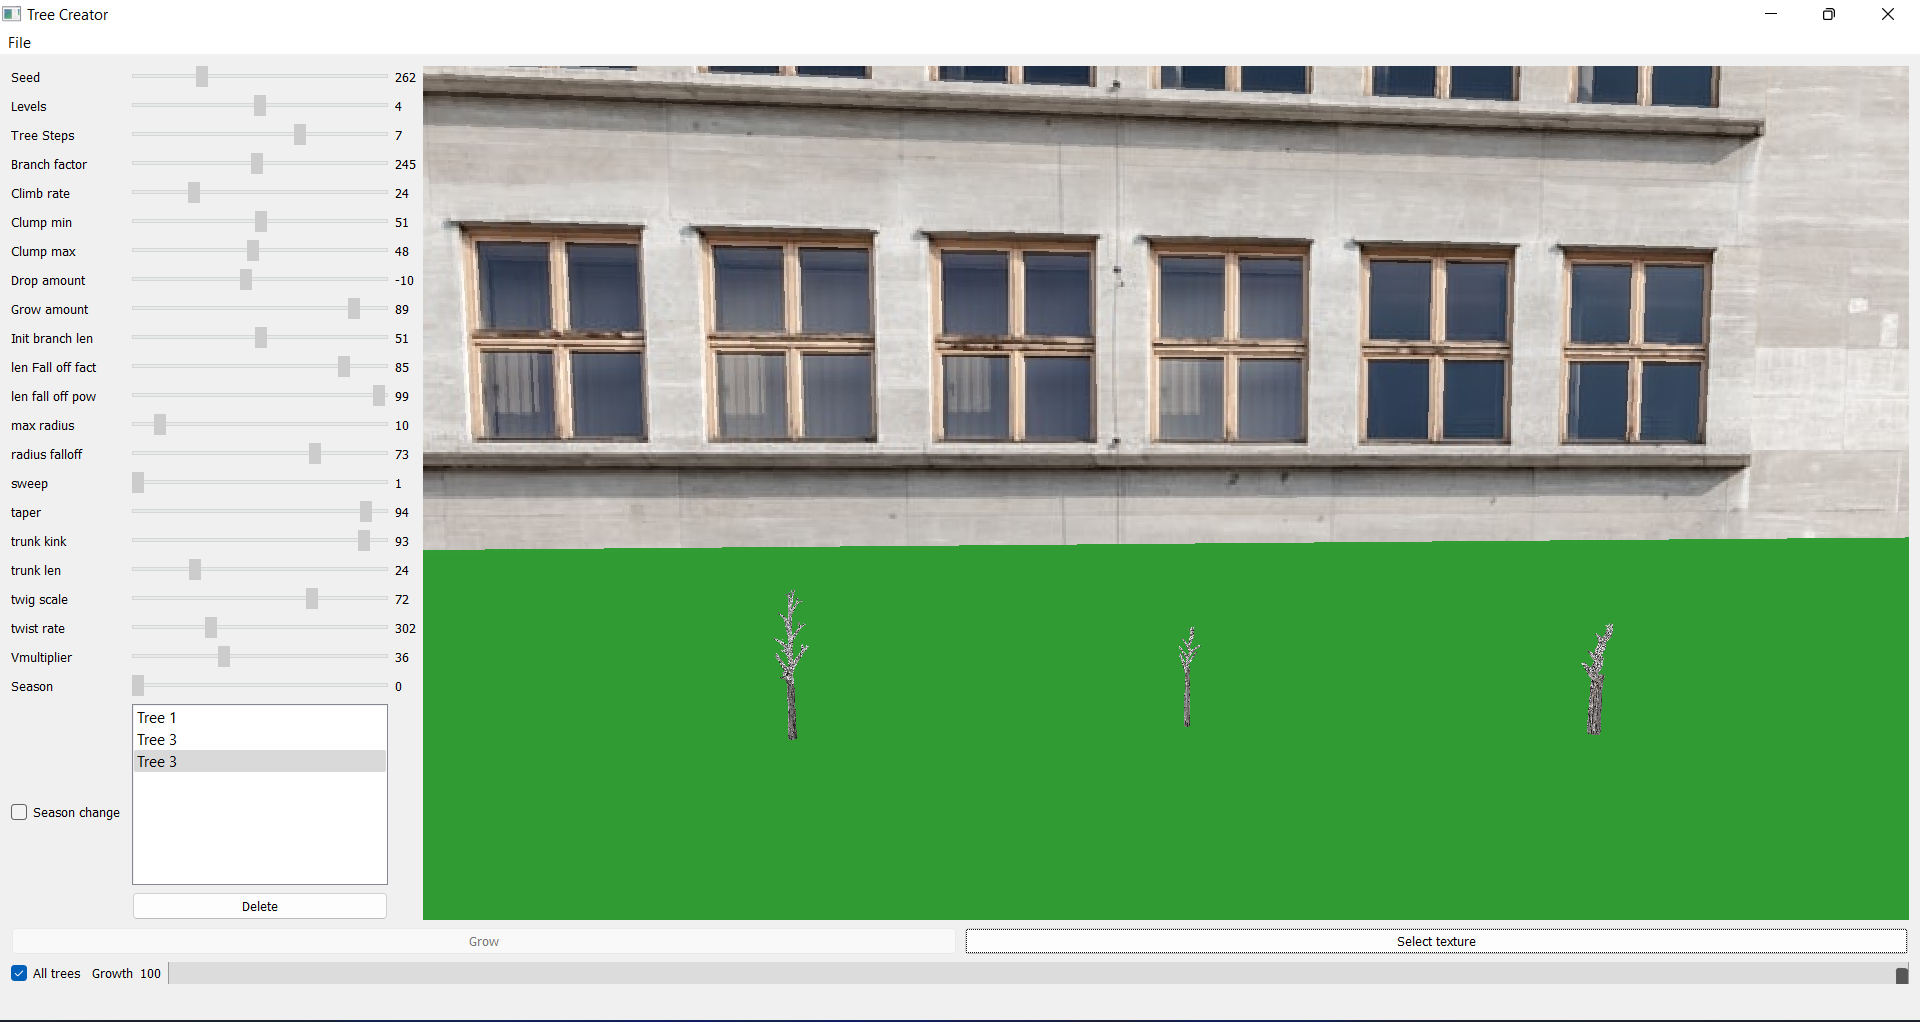
\includegraphics[width=15.5cm]{grafika/program/grow2.png}
% 	\caption{Automatyczny wzrost drzew}
%     \label{fig:grow2}
% \end{figure}

% \begin{figure}[H]
% 	\centering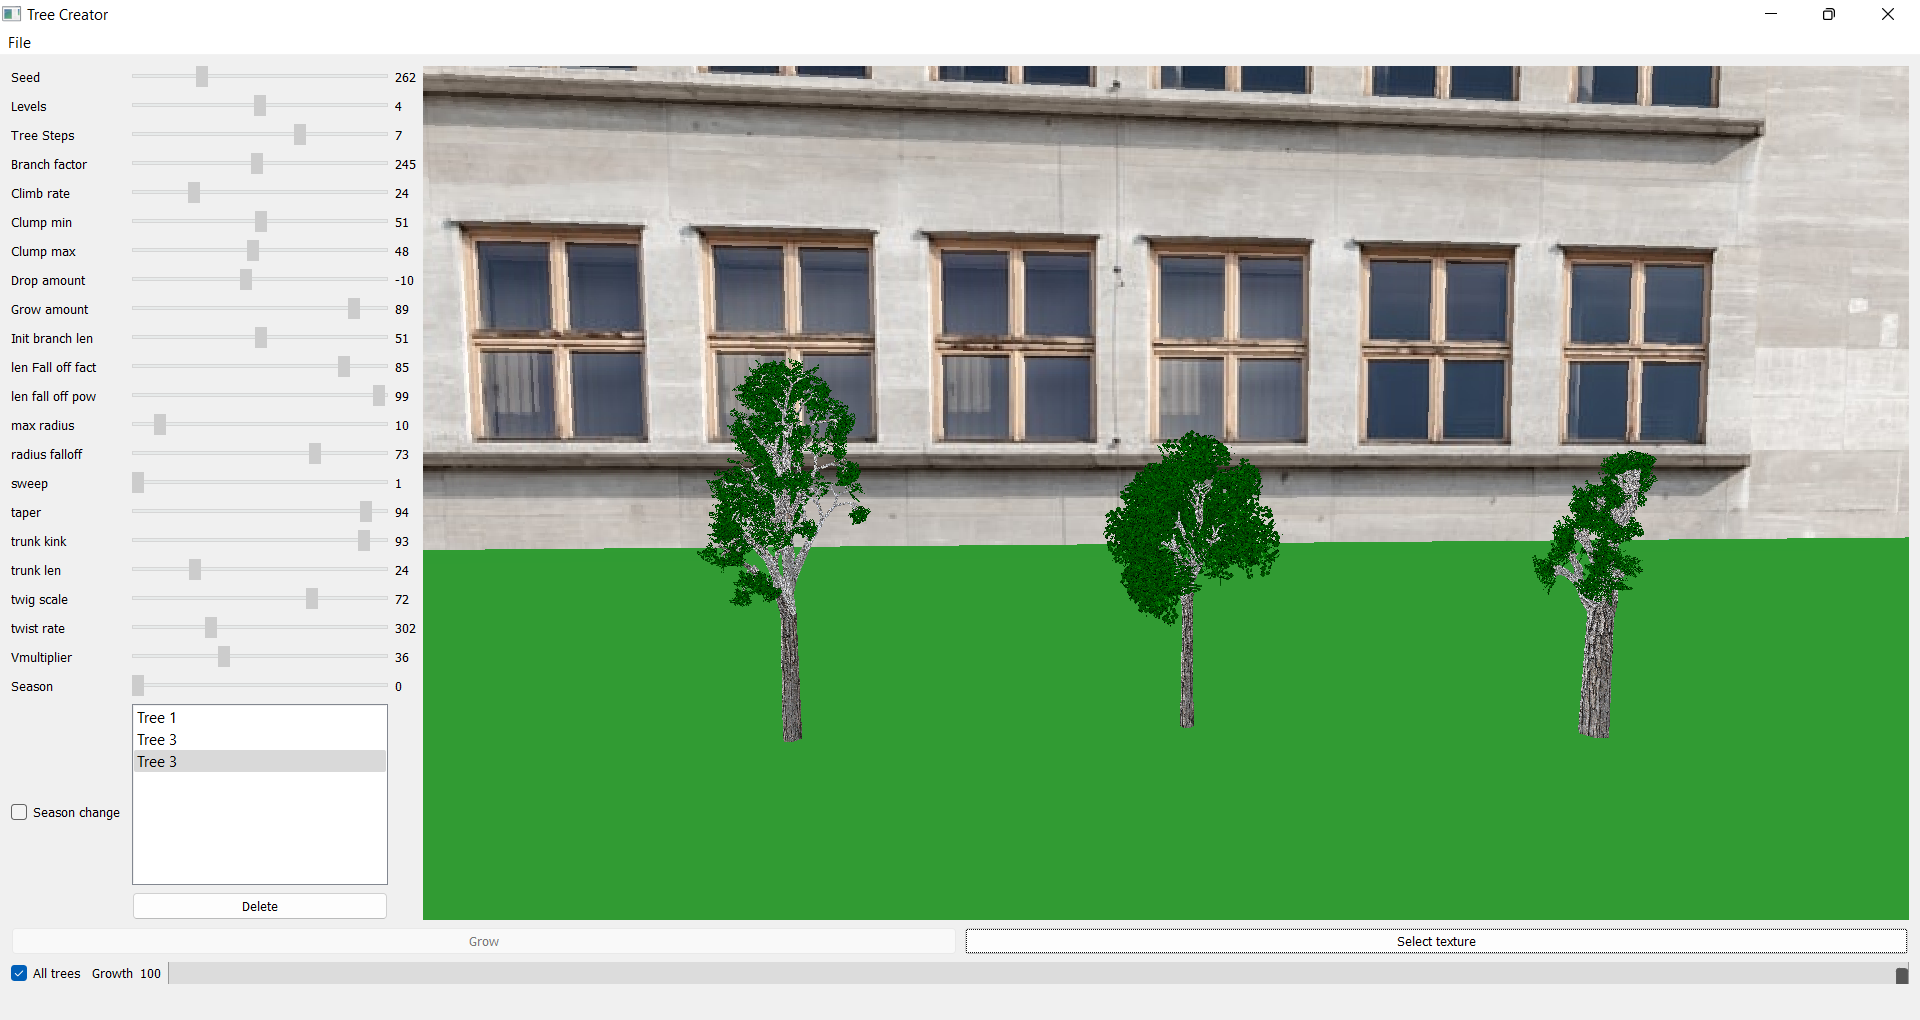
\includegraphics[width=15.5cm]{grafika/program/grow3.png}
% 	\caption{Automatyczny wzrost drzew}
%     \label{fig:grow3}
% \end{figure}


% \begin{figure}[H]
% 	\centering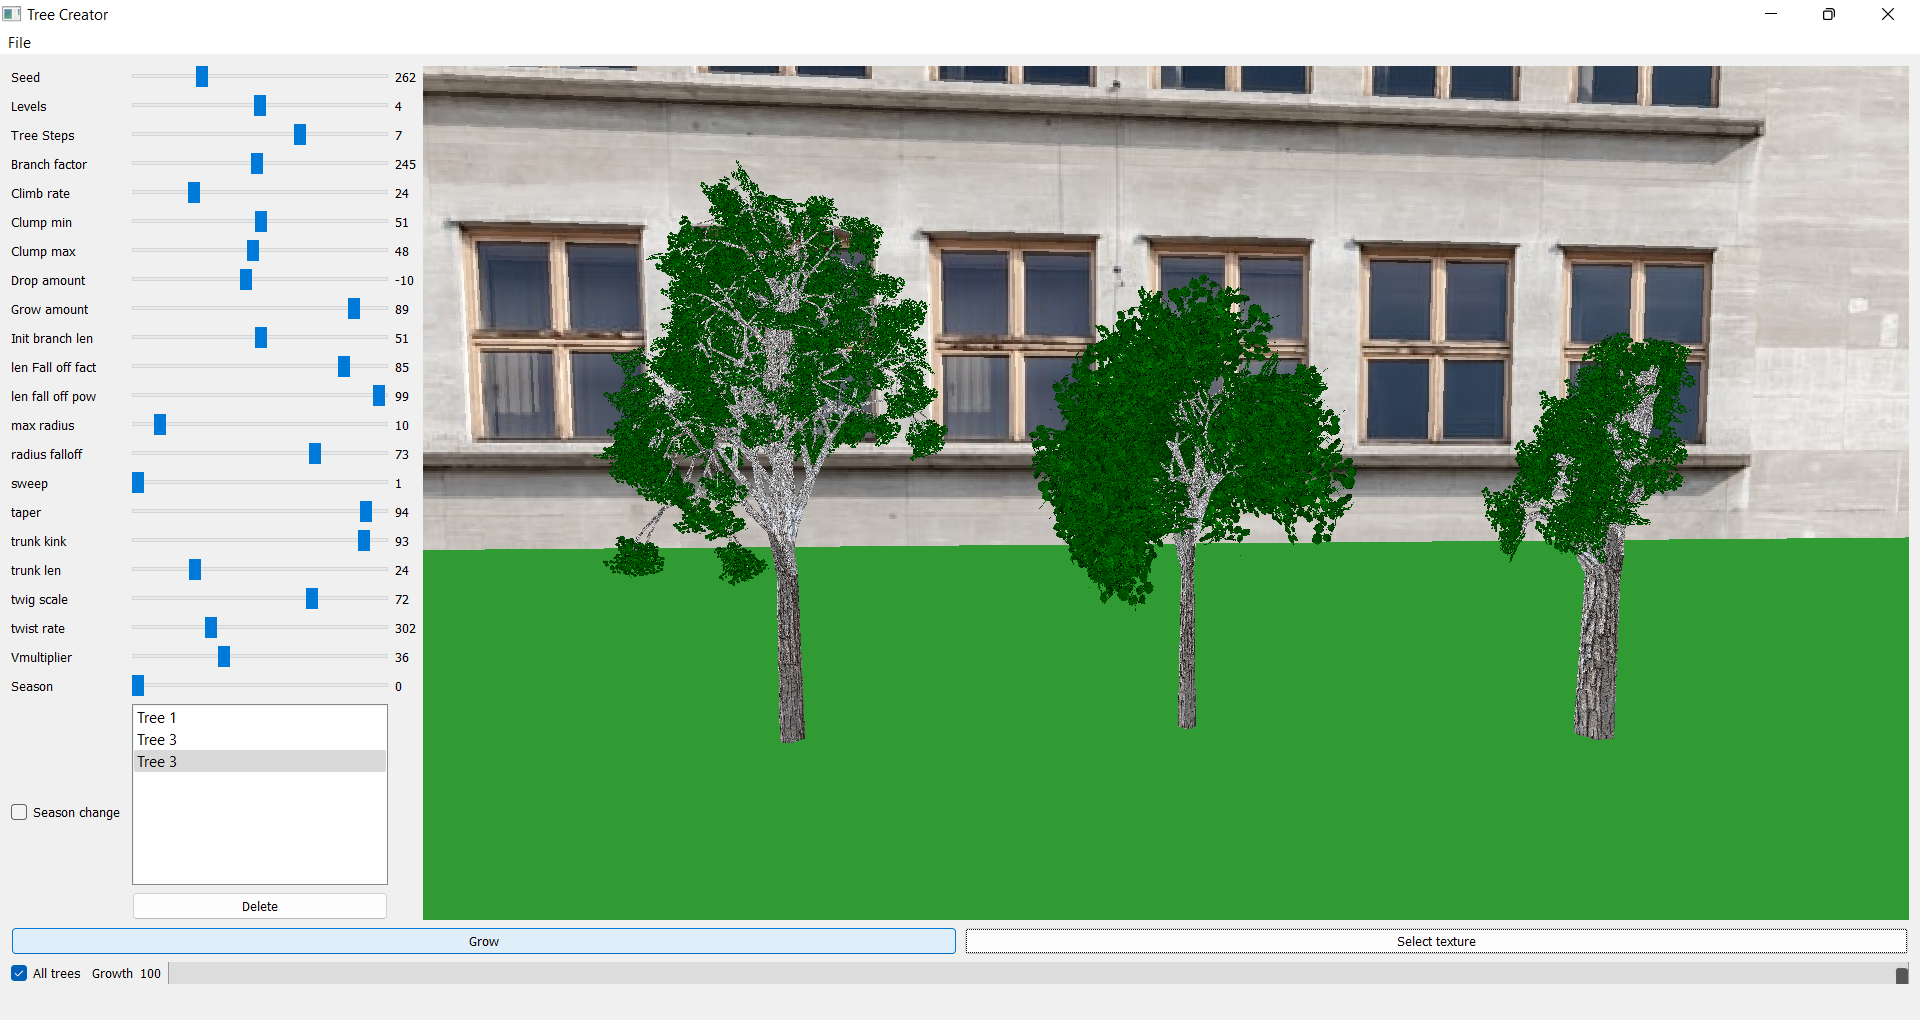
\includegraphics[width=15.5cm]{grafika/program/grow4.png}
% 	\caption{Koniec automatycznego wzrostu drzew}
%     \label{fig:grow4}
% \end{figure}

\begin{figure}[H]
	\centering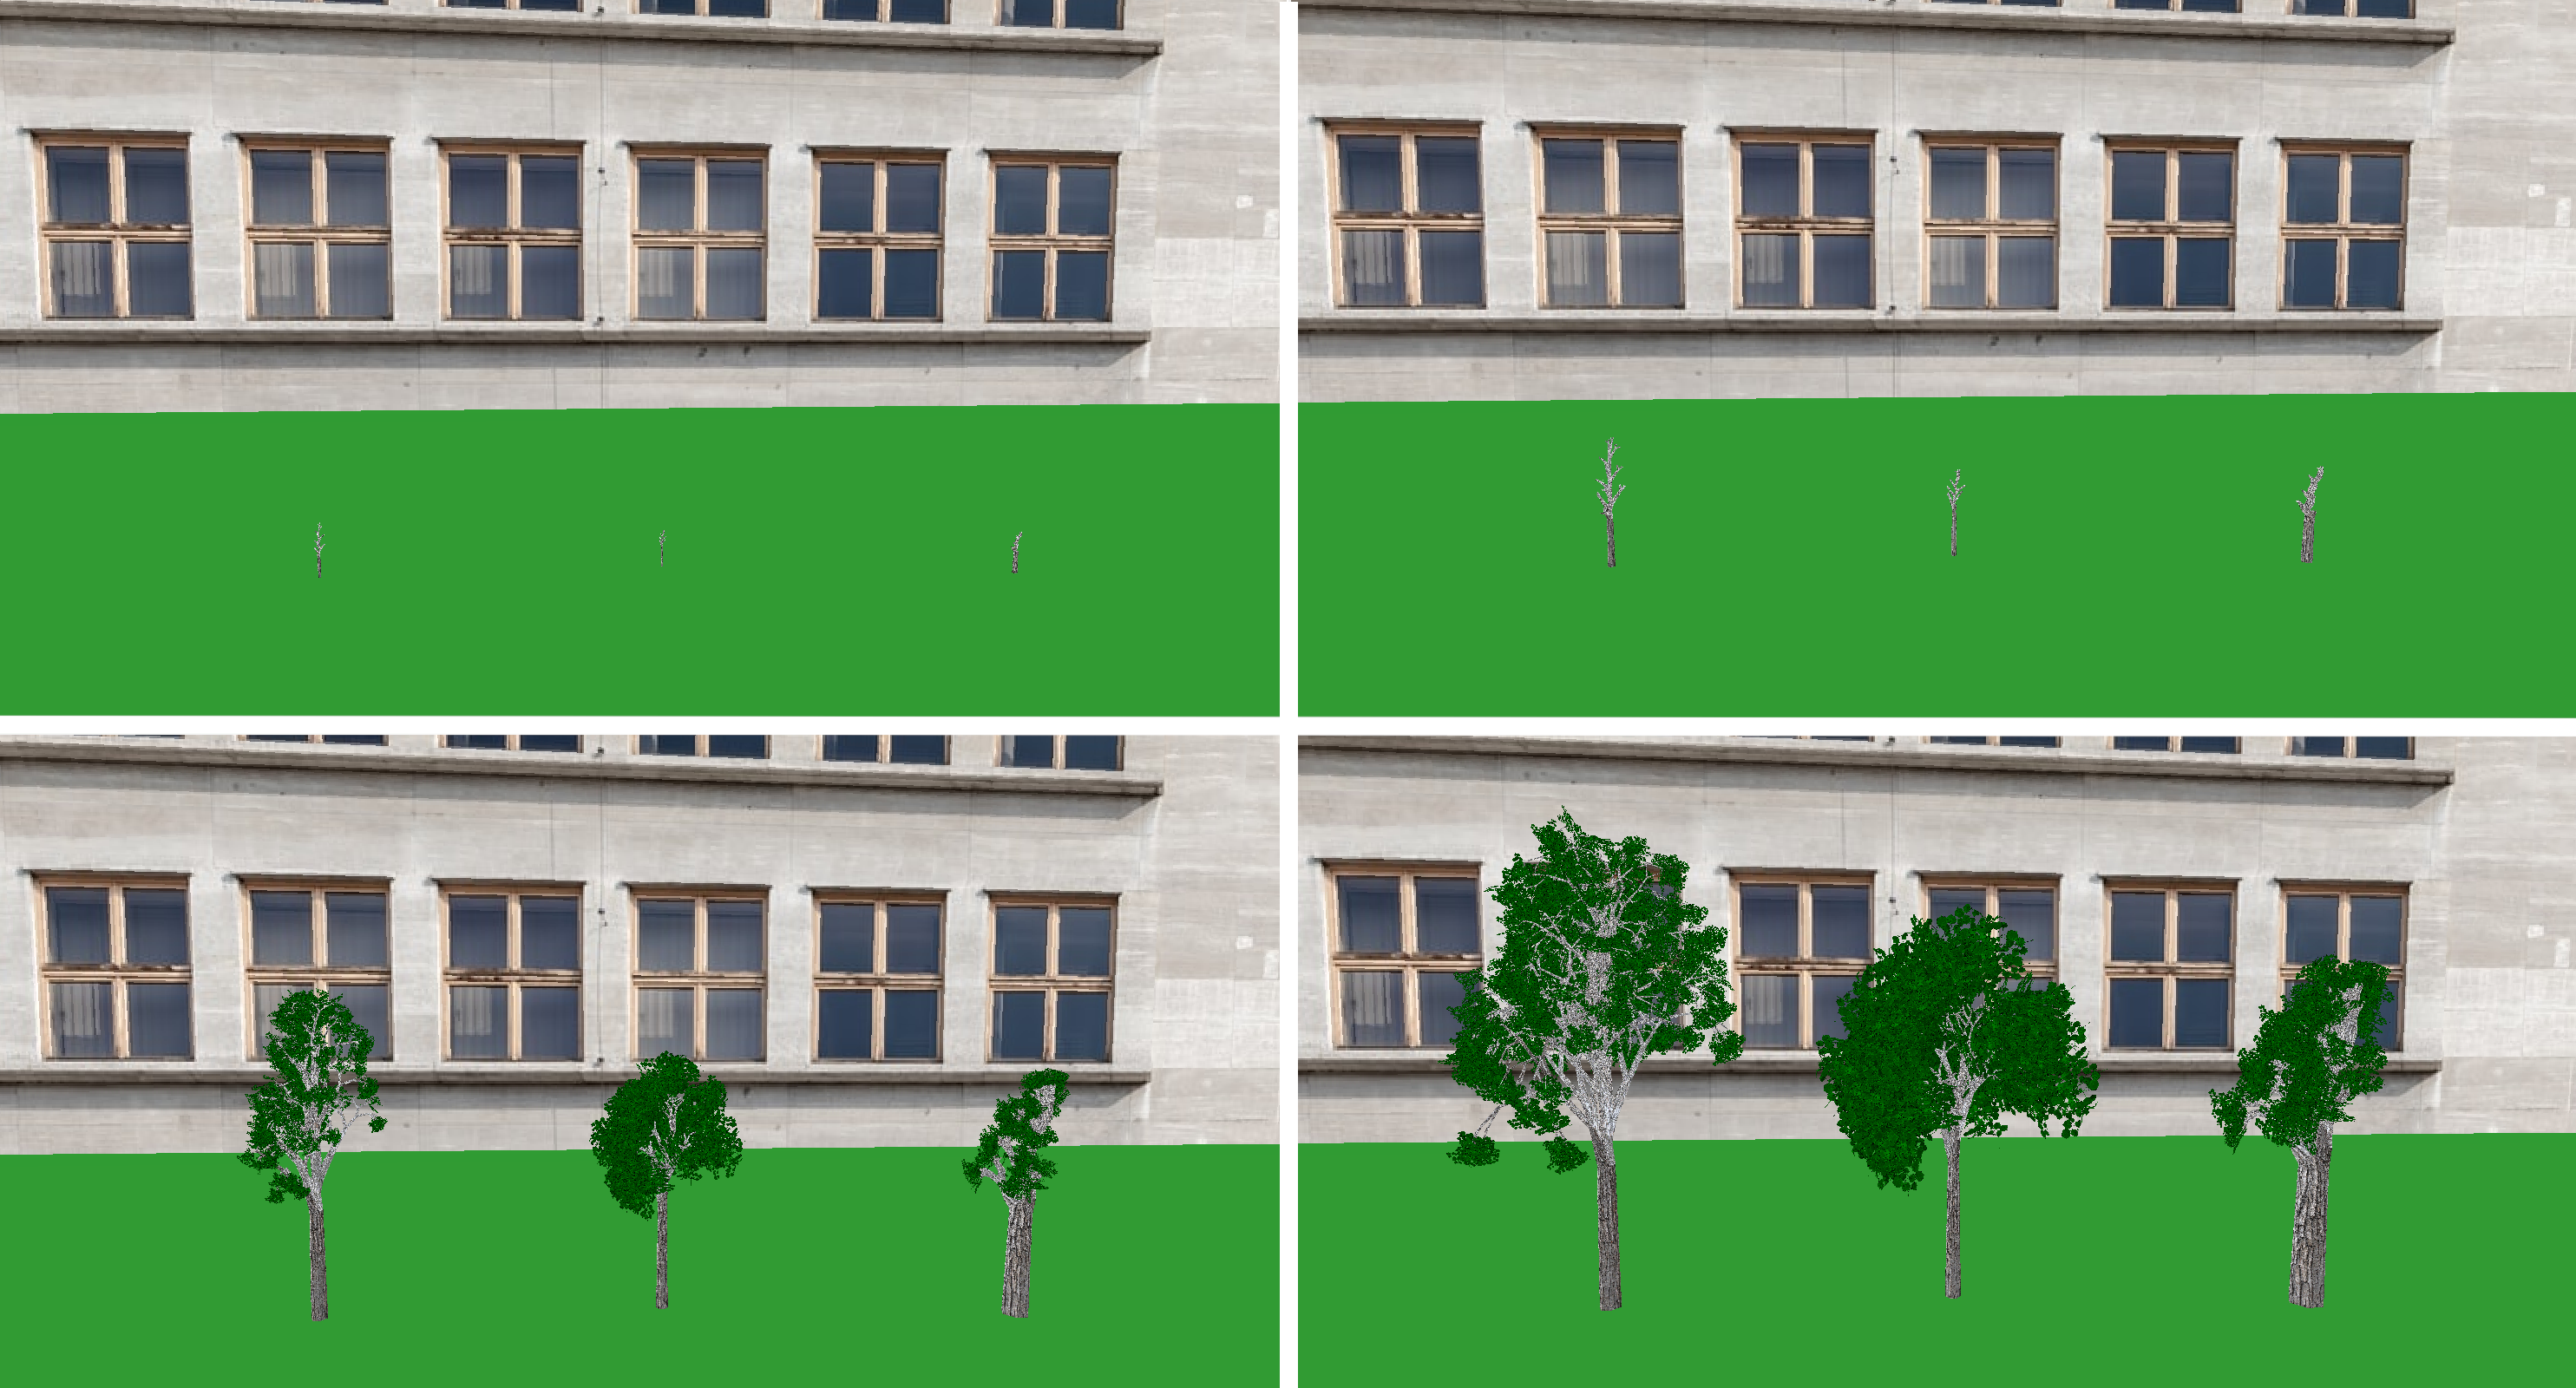
\includegraphics[width=15.5cm]{grafika/program/AllGrow.png}
	\caption{Automatyczny wzrost drzew}
    \label{fig:growAll}
\end{figure}

\textcolor{red}{Nie wiem czy 
lepiej robić każdy rysunek z \ref{fig:growAll} osobno, 
czy w jednym. Chyba tak jak jest (w jednym) będzie lepiej}

Liczba drzew wpływa na to, jak szybko będą generowane. 
Dzieje się tak dlatego, że każde drzewo jest generowane inaczej, 
biorąc pod uwagę to, jak będzie wyglądało pod koniec wzrostu.
Nie udało mi się tego zoptymalizować.

Podczas zmiany wzrostu można również poruszać kamerą, 
ale ponieważ proces wzrostu wymaga dość dużej wydajności, 
kamera może poruszać się wolniej.



\subsection{Ustawianie parametrów}

\subsection{Ustawianie tekstur}

\subsection{Zapis do pliku}

\section{Struktura programu}

\chapter{Testy i rezultaty}

\section{Wydajność}

\section{Porównanie z innymi rozwiązaniami}

\chapter{Podsumowanie}


\bibliographystyle{ieeetr}
\bibliography{bibliography/bib}
\addcontentsline{toc}{chapter}{Bibliografia}

\end{document}